\documentclass[12pt,a4paper]{article}
\usepackage[utf8]{inputenc}
\usepackage[T1]{fontenc}
\usepackage[spanish]{babel}
\usepackage{amsmath}
\usepackage{amsfonts}
\usepackage{enumitem}%separacion de las listas
\setlist[itemize]{noitemsep, topsep=1pt}%separacion de las listas
\setlist[enumerate]{noitemsep, topsep=1pt}%separacion de las listas

 %%%%%%%%%%%%%%%%%%%%%%%%%%%%%%%%%%%%%%%%%%%%%%%%%%%%%%%%%%%%%%%%%%%%%%%%%%%%%%%% 
%%% ~ Arduino Language - Arduino IDE Colors ~                                  %%%
%%%                                                                            %%%
%%% Kyle Rocha-Brownell | 10/2/2017 | No Licence                               %%%
%%% -------------------------------------------------------------------------- %%%
%%%                                                                            %%%
%%% Place this file in your working directory (next to the latex file you're   %%%
%%% working on).  To add it to your project, place:                            %%%
%%%    \input{arduinoLanguage.tex}                                             %%%
%%% somewhere before \begin{document} in your latex file.                      %%%
%%%                                                                            %%%
%%% In your document, place your arduino code between:                         %%%
%%%   \begin{lstlisting}[language=Arduino]                                     %%%
%%% and:                                                                       %%%
%%%   \end{lstlisting}                                                         %%%
%%%                                                                            %%%
%%% Or create your own style to add non-built-in functions and variables.      %%%
%%%                                                                            %%%
%%%%%%%%%%%%%%%%%%%%%%%%%%%%%%%%%%%%%%%%%%%%%%%%%%%%%%%%%%%%%%%%%%%%%%%%%%%%%%%% 

\usepackage{color}
\usepackage{listings}    
\usepackage{courier}


%%% Define Custom IDE Colors %%%
\definecolor{arduinoGreen}    {rgb} {0.17, 0.43, 0.01}
\definecolor{arduinoGrey}     {rgb} {0.47, 0.47, 0.33}
\definecolor{arduinoOrange}   {rgb} {0.8 , 0.4 , 0   }
\definecolor{arduinoBlue}     {rgb} {0.01, 0.61, 0.98}
\definecolor{arduinoDarkBlue} {rgb} {0.0 , 0.2 , 0.5 }

%%% Define Arduino Language %%%
\lstdefinelanguage{Arduino}{
	language=C++, % begin with default C++ settings 
	%
	%
	%%% Keyword Color Group 1 %%%  (called KEYWORD3 by arduino)
	keywordstyle=\color{arduinoGreen},   
	deletekeywords={  % remove all arduino keywords that might be in c++
		break, case, override, final, continue, default, do, else, for, 
		if, return, goto, switch, throw, try, while, setup, loop, export, 
		not, or, and, xor, include, define, elif, else, error, if, ifdef, 
		ifndef, pragma, warning,
		HIGH, LOW, INPUT, INPUT_PULLUP, OUTPUT, DEC, BIN, HEX, OCT, PI, 
		HALF_PI, TWO_PI, LSBFIRST, MSBFIRST, CHANGE, FALLING, RISING, 
		DEFAULT, EXTERNAL, INTERNAL, INTERNAL1V1, INTERNAL2V56, LED_BUILTIN, 
		LED_BUILTIN_RX, LED_BUILTIN_TX, DIGITAL_MESSAGE, FIRMATA_STRING, 
		ANALOG_MESSAGE, REPORT_DIGITAL, REPORT_ANALOG, SET_PIN_MODE, 
		SYSTEM_RESET, SYSEX_START, auto, int8_t, int16_t, int32_t, int64_t, 
		uint8_t, uint16_t, uint32_t, uint64_t, char16_t, char32_t, operator, 
		enum, delete, bool, boolean, byte, char, const, false, float, double, 
		null, NULL, int, long, new, private, protected, public, short, 
		signed, static, volatile, String, void, true, unsigned, word, array, 
		sizeof, dynamic_cast, typedef, const_cast, struct, static_cast, union, 
		friend, extern, class, reinterpret_cast, register, explicit, inline, 
		_Bool, complex, _Complex, _Imaginary, atomic_bool, atomic_char, 
		atomic_schar, atomic_uchar, atomic_short, atomic_ushort, atomic_int, 
		atomic_uint, atomic_long, atomic_ulong, atomic_llong, atomic_ullong, 
		virtual, PROGMEM,
		Serial, Serial1, Serial2, Serial3, SerialUSB, Keyboard, Mouse,
		abs, acos, asin, atan, atan2, ceil, constrain, cos, degrees, exp, 
		floor, log, map, max, min, radians, random, randomSeed, round, sin, 
		sq, sqrt, tan, pow, bitRead, bitWrite, bitSet, bitClear, bit, 
		highByte, lowByte, analogReference, analogRead, 
		analogReadResolution, analogWrite, analogWriteResolution, 
		attachInterrupt, detachInterrupt, digitalPinToInterrupt, delay, 
		delayMicroseconds, digitalWrite, digitalRead, interrupts, millis, 
		micros, noInterrupts, noTone, pinMode, pulseIn, pulseInLong, shiftIn, 
		shiftOut, tone, yield, Stream, begin, end, peek, read, print, 
		println, available, availableForWrite, flush, setTimeout, find, 
		findUntil, parseInt, parseFloat, readBytes, readBytesUntil, readString, 
		readStringUntil, trim, toUpperCase, toLowerCase, charAt, compareTo, 
		concat, endsWith, startsWith, equals, equalsIgnoreCase, getBytes, 
		indexOf, lastIndexOf, length, replace, setCharAt, substring, 
		toCharArray, toInt, press, release, releaseAll, accept, click, move, 
		isPressed, isAlphaNumeric, isAlpha, isAscii, isWhitespace, isControl, 
		isDigit, isGraph, isLowerCase, isPrintable, isPunct, isSpace, 
		isUpperCase, isHexadecimalDigit, 
	}, 
	morekeywords={   % add arduino structures to group 1
		break, case, override, final, continue, default, do, else, for, 
		if, return, goto, switch, throw, try, while, setup, loop, export, 
		not, or, and, xor, include, define, elif, else, error, if, ifdef, 
		ifndef, pragma, warning,
	}, 
	% 
	%
	%%% Keyword Color Group 2 %%%  (called LITERAL1 by arduino)
	keywordstyle=[2]\color{arduinoBlue},   
	keywords=[2]{   % add variables and dataTypes as 2nd group  
		HIGH, LOW, INPUT, INPUT_PULLUP, OUTPUT, DEC, BIN, HEX, OCT, PI, 
		HALF_PI, TWO_PI, LSBFIRST, MSBFIRST, CHANGE, FALLING, RISING, 
		DEFAULT, EXTERNAL, INTERNAL, INTERNAL1V1, INTERNAL2V56, LED_BUILTIN, 
		LED_BUILTIN_RX, LED_BUILTIN_TX, DIGITAL_MESSAGE, FIRMATA_STRING, 
		ANALOG_MESSAGE, REPORT_DIGITAL, REPORT_ANALOG, SET_PIN_MODE, 
		SYSTEM_RESET, SYSEX_START, auto, int8_t, int16_t, int32_t, int64_t, 
		uint8_t, uint16_t, uint32_t, uint64_t, char16_t, char32_t, operator, 
		enum, delete, bool, boolean, byte, char, const, false, float, double, 
		null, NULL, int, long, new, private, protected, public, short, 
		signed, static, volatile, String, void, true, unsigned, word, array, 
		sizeof, dynamic_cast, typedef, const_cast, struct, static_cast, union, 
		friend, extern, class, reinterpret_cast, register, explicit, inline, 
		_Bool, complex, _Complex, _Imaginary, atomic_bool, atomic_char, 
		atomic_schar, atomic_uchar, atomic_short, atomic_ushort, atomic_int, 
		atomic_uint, atomic_long, atomic_ulong, atomic_llong, atomic_ullong, 
		virtual, PROGMEM,
	},  
	% 
	%
	%%% Keyword Color Group 3 %%%  (called KEYWORD1 by arduino)
	keywordstyle=[3]\bfseries\color{arduinoOrange},
	keywords=[3]{  % add built-in functions as a 3rd group
		Serial, Serial1, Serial2, Serial3, SerialUSB, Keyboard, Mouse,
	},      
	%
	%
	%%% Keyword Color Group 4 %%%  (called KEYWORD2 by arduino)
	keywordstyle=[4]\color{arduinoOrange},
	keywords=[4]{  % add more built-in functions as a 4th group
		abs, acos, asin, atan, atan2, ceil, constrain, cos, degrees, exp, 
		floor, log, map, max, min, radians, random, randomSeed, round, sin, 
		sq, sqrt, tan, pow, bitRead, bitWrite, bitSet, bitClear, bit, 
		highByte, lowByte, analogReference, analogRead, 
		analogReadResolution, analogWrite, analogWriteResolution, 
		attachInterrupt, detachInterrupt, digitalPinToInterrupt, delay, 
		delayMicroseconds, digitalWrite, digitalRead, interrupts, millis, 
		micros, noInterrupts, noTone, pinMode, pulseIn, pulseInLong, shiftIn, 
		shiftOut, tone, yield, Stream, begin, end, peek, read, print, 
		println, available, availableForWrite, flush, setTimeout, find, 
		findUntil, parseInt, parseFloat, readBytes, readBytesUntil, readString, 
		readStringUntil, trim, toUpperCase, toLowerCase, charAt, compareTo, 
		concat, endsWith, startsWith, equals, equalsIgnoreCase, getBytes, 
		indexOf, lastIndexOf, length, replace, setCharAt, substring, 
		toCharArray, toInt, press, release, releaseAll, accept, click, move, 
		isPressed, isAlphaNumeric, isAlpha, isAscii, isWhitespace, isControl, 
		isDigit, isGraph, isLowerCase, isPrintable, isPunct, isSpace, 
		isUpperCase, isHexadecimalDigit, 
	},      
	%
	%
	%%% Set Other Colors %%%
	stringstyle=\color{arduinoDarkBlue},    
	commentstyle=\color{arduinoGrey},    
	%          
	%   
	%%%% Line Numbering %%%%
	numbers=left,                    
	numbersep=5pt,                   
	numberstyle=\color{arduinoGrey}\scriptsize,    
	xleftmargin=10pt,
	stepnumber=2,           
	lineskip=-0.5ex,           % show every 2 line numbers
	%
	%
	%%%% Code Box Style %%%%
	breaklines=true,                    % wordwrapping
	tabsize=2,         
	basicstyle=\footnotesize\ttfamily
}%biblioteca de codigos
\usepackage{verbatim}
\usepackage{listings}
\usepackage{color}

% Processing language definition template for LaTeX listings package v1.2
%
% Credits to ebigunso for creating this LaTeX listings language definition template for Processing
% This template is licensed with CreativeCommons license CC-BY-SA 4.0
% license info:
% https://creativecommons.org/licenses/by-sa/4.0/legalcode

%Define Colors
\definecolor{black}{RGB}{0,0,0}
\definecolor{gray}{RGB}{102,102,102}		%#666666
\definecolor{function}{RGB}{0,102,153}		%#006699 lightblue
\definecolor{lightgreen}{RGB}{102,153,0}	%#669900
\definecolor{bluegreen}{RGB}{51,153,126}	%#33997e
\definecolor{magenta}{RGB}{217,74,122}	%#d94a7a
\definecolor{orange}{RGB}{226,102,26}		%#e2661a
\definecolor{purple}{RGB}{125,71,147}		%#7d4793
\definecolor{green}{RGB}{113,138,98}		%#718a62

\lstdefinelanguage{Processing}{
	%keyword1&2&6
	morekeywords = [3]{abstract, break, class, continue, default, enum, extends, false, final, finally, implements, import, instanceof, interface, native, new, null, package, private, protected, public, static, strictfp, throws, transient, true, void, volatile, length, assert, case, return, super, this, throw},
	%keyword3
	morekeywords = [4]{catch, do, for, if, else, switch, synchronized, while, try},
	%keyword4
	morekeywords = [5]{width, height, pixelHeight, displayHeight, displayWidth, focused, frameCount, frameRate, key, keyCode, keyPressed, mouseButton, mousePressed, mouseX, mouseY, pixels, pixelWidth, pmouseX, pmouseY},
	%keyword5
	morekeywords = [6]{Array, ArrayList, Boolean, Byte, BufferedReader, Character, Class, Double, Float, Integer, HashMap, PrintWriter, String, StringBuffer, StringBuilder, Thread, boolean, byte, char, color, double, float, int, long, short, FloatDict, FloatList, IntDict, IntList, JSONArray, JSONObject, PFont, PGraphics, PImage, PShader, PShape, PVector, StringDict, StringList, Table, TableRow, XML},
	%literal2
	morekeywords = [7]{ADD, ALIGN_CENTER, ALIGN_LEFT, ALIGN_RIGHT, ALPHA, ALPHA_MASK, ALT, AMBIENT, ARC, ARROW, ARGB, BACKSPACE, BASELINE, BEVEL, BLEND, BLUE_MASK, BLUR, BOTTOM, BOX, BURN, CENTER, CHATTER, CHORD, CLAMP, CLICK, CLOSE, CMYK, CODED, COMPLAINT, COMPOSITE, COMPONENT, CONCAVE_POLYGON, CONTROL, CONVEX_POLYGON, CORNER, CORNERS, CROSS, CUSTOM, DARKEST, DEGREES, DEG_TO_RAD, DELETE, DIAMETER, DIFFERENCE, DIFFUSE, DILATE, DIRECTIONAL, DISABLE_ACCURATE_2D, DISABLE_DEPTH_MASK, DISABLE_DEPTH_SORT, DISABLE_DEPTH_TEST, DISABLE_NATIVE_FONTS, DISABLE_OPENGL_ERRORS, DISABLE_PURE_STROKE, DISABLE_TEXTURE_MIPMAPS, DISABLE_TRANSFORM_CACHE, DISABLE_STROKE_PERSPECTIVE, DISABLED, DODGE, DOWN, DRAG, DXF, ELLIPSE, ENABLE_ACCURATE_2D, ENABLE_DEPTH_MASK, ENABLE_DEPTH_SORT, ENABLE_DEPTH_TEST, ENABLE_NATIVE_FONTS, ENABLE_OPENGL_ERRORS, ENABLE_PURE_STROKE, ENABLE_TEXTURE_MIPMAPS, ENABLE_TRANSFORM_CACHE, ENABLE_STROKE_PERSPECTIVE, ENTER, EPSILON, ERODE, ESC, EXCLUSION, EXIT, FX2D, GIF, GRAY, GREEN_MASK, GROUP, HALF, HALF_PI, HAND, HARD_LIGHT, HINT_COUNT, HSB, IMAGE, INVERT, JAVA2D, JPEG, LEFT, LIGHTEST, LINE, LINES, LINUX, MACOSX, MAX_FLOAT, MAX_INT, MIN_FOAT, MIN_INT, MITER, MODEL, MOVE, MULTIPLY, NORMAL, NORMALIZED, NO_DEPTH_TEST, NTSC, ONE, OPAQUE, OPEN, ORTHOGRAPHIC, OVERLAY, PAL, PDF, P2D, P3D, PERSPECTIVE, PI, PIE, PIXEL_CENTER, POINT, POINTS, POSTERIZE, PRESS, PROBLEM, PROJECT, QUAD, QUAD_STRIP, QUADS, QUARTER_PI, RAD_TO_DEG, RADIUS, RADIANS, RECT, RED_MASK, RELEASE, REPEAT, REPLACE, RETURN, RGB, RIGHT, ROUND, SCREEN, SECAM, SHAPE, SHIFT, SPAN, SPECULAR, SPHERE, SOFT_LIGHT, SQUARE, SUBTRACT, SVG, SVIDEO, TAB, TARGA, TAU, TEXT, TFF, THIRD_PI, THRESHOLD, TIFF, TOP, TRIANGLE, TRIANGLE_FAN, TRIANGLES, TRIANGLE_STRIP, TUNER, TWO, TWO_PI, UP, WAIT, WHITESPACE},
	%function1
	morekeywords = [8]{start, stop, breakShape, createPath, loadMatrix, parseBoolean, parseByte, parseChar, parseFloat, parseInt, saveFile, savePath, sketchFile, sketchPath, abs, acos, alpha, ambient, ambientLight, append, applyMatrix, arc, arrayCopy, asin, atan, atan2, background, beginCamera, beginContour, beginRaw, beginRecord, beginShape, bezier, bezierDetail, bezierPoint, bezierTangent, bezierVertex, binary, blend, blendColor, blendMode, blue, box, brightness, camera, ceil, circle, clear, clip, color, colorMode, concat, constrain, copy, cos, createFont, createGraphics, createImage, createInput, createOutput, createReader, createShape, createWriter, cursor, curve, curveDetail, curvePoint, curveTangent, curveTightness, curveVertex, day, degrees, delay, directionalLight, displayDensity, dist, ellipse, ellipseMode, emissive, endCamera, endContour, endRaw, endRecord, endShape, exit, exp, expand, fill, filter, floor, frustum, fullScreen, get, green, hex, hint, hour, hue, image, imageMode, join, launch, lerp, lerpColor, lightFalloff, lights, lightSpecular, line, loadBytes, loadFont, loadImage, loadJSONArray, loadJSONObject, loadPixels, loadShader, loadShape, loadStrings, loadTable, loadXML, log, loop, mag, map, match, matchAll, max, millis, min, minute, modelX, modelY, modelZ, month, nf, nfc, nfp, nfs, noClip, noCursor, noFill, noise, noiseDetail, noiseSeed, noLights, noLoop, norm, normal, noSmooth, noStroke, noTint, ortho, parseJSONArray, parseJSONObject, parseXML, perspective, list, pixelDensity, point, pointLight, popMatrix, popStyle, pow, print, printArray, printCamera, println, printMatrix, printProjection, pushMatrix, pushStyle, quad, quadraticVertex, radians, random, randomGaussian, randomSeed, rect, rectMode, red, redraw, requestImage, resetMatrix, resetShader, reverse, rotate, rotateX, rotateY, rotateZ, round, saturation, save, saveBytes, saveFrame, saveJSONArray, saveJSONObject, saveStream, saveStrings, saveTable, saveXML, scale, screenX, screenY, screenZ, second, selectFolder, selectInput, selectOutput, set, shader, shape, shapeMode, shearX, shearY, shininess, shorten, sin, size, smooth, sort, specular, sphere, sphereDetail, splice, split, splitTokens, spotLight, sq, sqrt, square, stroke, strokeCap, strokeJoin, strokeWeight, subset, tan, text, textAlign, textAscent, textDescent, textFont, textLeading, textMode, textSize, texture, textureMode, textureWrap, textWidth, thread, tint, translate, triangle, trim, unbinary, unhex, updatePixels, vertex, year},
	%function2
	morekeywords = [9]{cache, readLine, close, flush, print, println, charAt, equals, indexOf, substring, toLowerCase, toUpperCase, getDouble, getLong, getColumnTitles, getColumnTypes, getColumnType, setDouble, setLong, add, clear, div, get, hasKey, keyArray, keys, mult, remove, set, size, sortKeys, sortKeysReverse, sortValues, sortValuesReverse, sub, valueArray, values, append, array, hasValue, max, min, mult, remove, reverse, shuffle, sort, sortReverse, increment, getBoolean, getFloat, getInt, getIntArray, getJSONArray, getJSONObject, getString, getStringArray, isNull, setBoolean, setFloat, setInt, setJSONArray, setJSONObject, setString, beginDraw, endDraw, blend, copy, filter, loadPixels, mask, resize, save, updatePixels, addChild, beginContour, beginShape, disableStyle, enableStyle, endContour, endShape, getChild, getChildCount, getVertex, getVertexCount, isVisible, resetMatrix, rotate, rotateX, rotateY, rotateZ, scale, setFill, setStroke, setVertex, setVisible, translate, angleBetween, cross, dist, dot, fromAngle, heading, lerp, limit, mag, magSq, normalize, random2D, random3D, setMag, lower, upper, addColumn, addRow, clearRows, findRow, findRows, getColumnCount, getRow, getRowCount, getStringColumn, matchRow, matchRows, removeColumn, removeRow, removeTokens, rows, trim, getColumnTitle, format, getAttributeCount, getChildren, getContent, getName, getParent, hasAttribute, hasChildren, listAttributes, listChildren, removeChild, setContent, setName, toString},
	%function4
	morekeywords = [10]{draw, keyReleased, keyTyped, mouseClicked, mouseDragged, mouseMoved, mouseReleased, mouseWheel, settings, setup},
	keywordstyle = [3]\color{bluegreen},
	keywordstyle = [4]\color{lightgreen},
	keywordstyle = [5]\color{magenta},
	keywordstyle = [6]\color{orange},
	keywordstyle = [7]\color{green},
	keywordstyle = [8]\color{function},
	keywordstyle = [9]\color{function},
	keywordstyle = [10]\color{function}\bfseries,
	sensitive = true,
	morecomment = [l][\color{gray}]{//},
	morecomment = [s][\color{gray}]{/*}{*/},
	morecomment = [s][\color{gray}]{/**}{*/},
	morestring = [b][\color{purple}]",
	morestring = [b][\color{purple}]'
}
\renewcommand{\ttdefault}{pcr}
\lstset{
	language={Processing},
	basicstyle={\small\ttfamily},
	identifierstyle={\small},
	commentstyle={\small\itshape},
	keywordstyle={\small},
	ndkeywordstyle={\small},
	stringstyle={\small\ttfamily},
	frame={tb},
	numbers=left,                    
	numbersep=5pt,                   
	numberstyle=\scriptsize,    
	xleftmargin=10pt,
	stepnumber=2,           
	lineskip=-0.5ex,           % show every 2 line numbers
	breaklines=true,                    % wordwrapping
	tabsize=2,         
	basicstyle=\footnotesize\ttfamily
%	columns=[l]{fullflexible},
%	numbers=left,
%	xrightmargin=0em,
%	xleftmargin=10pt,
%	numberstyle={\scriptsize},
%	firstnumber=1,
%	stepnumber=2,  
%	numbersep=5pt,
%	lineskip=-0.5ex,
}

\usepackage{appendix}
\renewcommand{\appendixpagename}{Anexos}

\usepackage{multirow} %tablas
\usepackage[table,xcdraw]{xcolor} %color tablas
\usepackage{hhline}

\usepackage{fancyhdr}%encabezado y pie de pagina

\usepackage{comment}
\usepackage{float} 
\usepackage{tcolorbox} %cajas con definiciones
\usepackage{graphicx}
\usepackage{caption}
\usepackage{wrapfig} %para imagen al lado de texto
\usepackage{color}%resaltador
\usepackage{soul}%resaltador
\usepackage[none]{hyphenat} %para que no corte las palabras al final del renglon
\usepackage{amssymb}
\usepackage{graphicx}
\usepackage{subfigure}
\usepackage{amssymb}%simbolos matematiacos
\usepackage{amsmath}%simbolos matematiacos
%%\usepackage{pstricks,pst-node}% diagrama en bloques

%reiniciar los contadores de figuras
\usepackage{chngcntr}
\counterwithin{figure}{section}
\counterwithin{table}{section}

\usepackage{url} %url
\usepackage{hyperref} %indice con hipervínculo
\hypersetup{
    colorlinks=true,
    linkcolor=blue,
    filecolor=white,      
    urlcolor=blue,
    citecolor=blue,
}

%bibliografía
\usepackage[maxbibnames=99, sorting=none, backend=bibtex]{biblatex}
\addbibresource{biblio.bib}
%\usepackage[nottoc]{biblatex}


%para crear sub sub sub titulos
\makeatletter
\renewcommand\paragraph{\@startsection{paragraph}{4}{\z@}%
            {-2.5ex\@plus -1ex \@minus -.25ex}%
            {1.25ex \@plus .25ex}%
            {\normalfont\normalsize\bfseries}}
\makeatother
\setcounter{secnumdepth}{4} % how many sectioning levels to assign numbers to
\setcounter{tocdepth}{4}    % how many sectioning levels to show in ToC

\usepackage[left=2.50cm, right=2.50cm, top=2.50cm, bottom=2.50cm]{geometry}
\author{Caamiña Quineros, Daniela Beatriz\\ \and Yapura, Cristian Alejandro}
\title{Proyecto final}
\graphicspath{ {imagenes/} }

\newcommand{\grad}{$^{\circ}$}

%encabezado y pie de pagina
\pagestyle{fancy}
\fancyhead[L]{}
\fancyhead[R]{}
\fancyhead[C]{\textbf{Automatización de Túnel de Viento}}
\fancyfoot[L]{}
\fancyfoot[C]{\thepage}
\fancyfoot[R]{Autores: Caamiña - Yapura}
\renewcommand{\headrulewidth}{0.4pt}
\renewcommand{\footrulewidth}{2pt}



\begin{document}
%	\maketitle

\begin{titlepage}
	\centering
	{
\includegraphics[width=0.2\textwidth]{unpsjb.png}\par}
	\vspace{1cm}
	{\bfseries\LARGE Universidad Nacional de la Patagonia\\ San Juan Bosco \par}
	\vspace{1cm}
	{\scshape\Large Facultad de Ingenier\'ia \par}
	\vspace{3cm}
	{\scshape\Huge Automatización de Túnel de Viento \par}
	\vspace{3cm}
	{\itshape\Large Proyecto Final de Carrera\\ - Ingeniería Electrónica - \par}
	\vfill
	{\Large Autores: \par}
	{\Large Caamiña Quineros, Daniela Beatriz\\ Yapura, Cristian Alejandro \par}
	\vfill
	{\Large Diciembre 2021 \par}
	\end{titlepage}



\newpage


\section*{Agradecimientos}
	
	\vspace{6cm}

 
		\begin{flushright}
	\textit{	Agradecemos a Gerardo, quien nos convocó para la realización de este proyecto y al Laboratorio de Mecánica de Fluidos que nos abrió las puertas para poder realizarlo.}\\
		\vspace{3cm}
	\textit{	Este proyecto está especialmente dedicado a nuestros padres quienes nos brindaron el apoyo y estuvieron en cada paso de nuestra carrera universitaria, también agradecemos infinitamente a nuestros hermanos, novia/o, familia y amigos quienes fueron nuestro soporte y que nos acompañaron durante todos los años de estudio. Reconocemos y agradecemos a cada persona que de alguna forma nos ayudó a transitar este camino.}
		\end{flushright}

	
	
		

\newpage
\vspace*{6cm}
\begin{flushright}
	...la foto del recuerdo
\end{flushright}
	
\begin{figure}[htb]
	\centering
	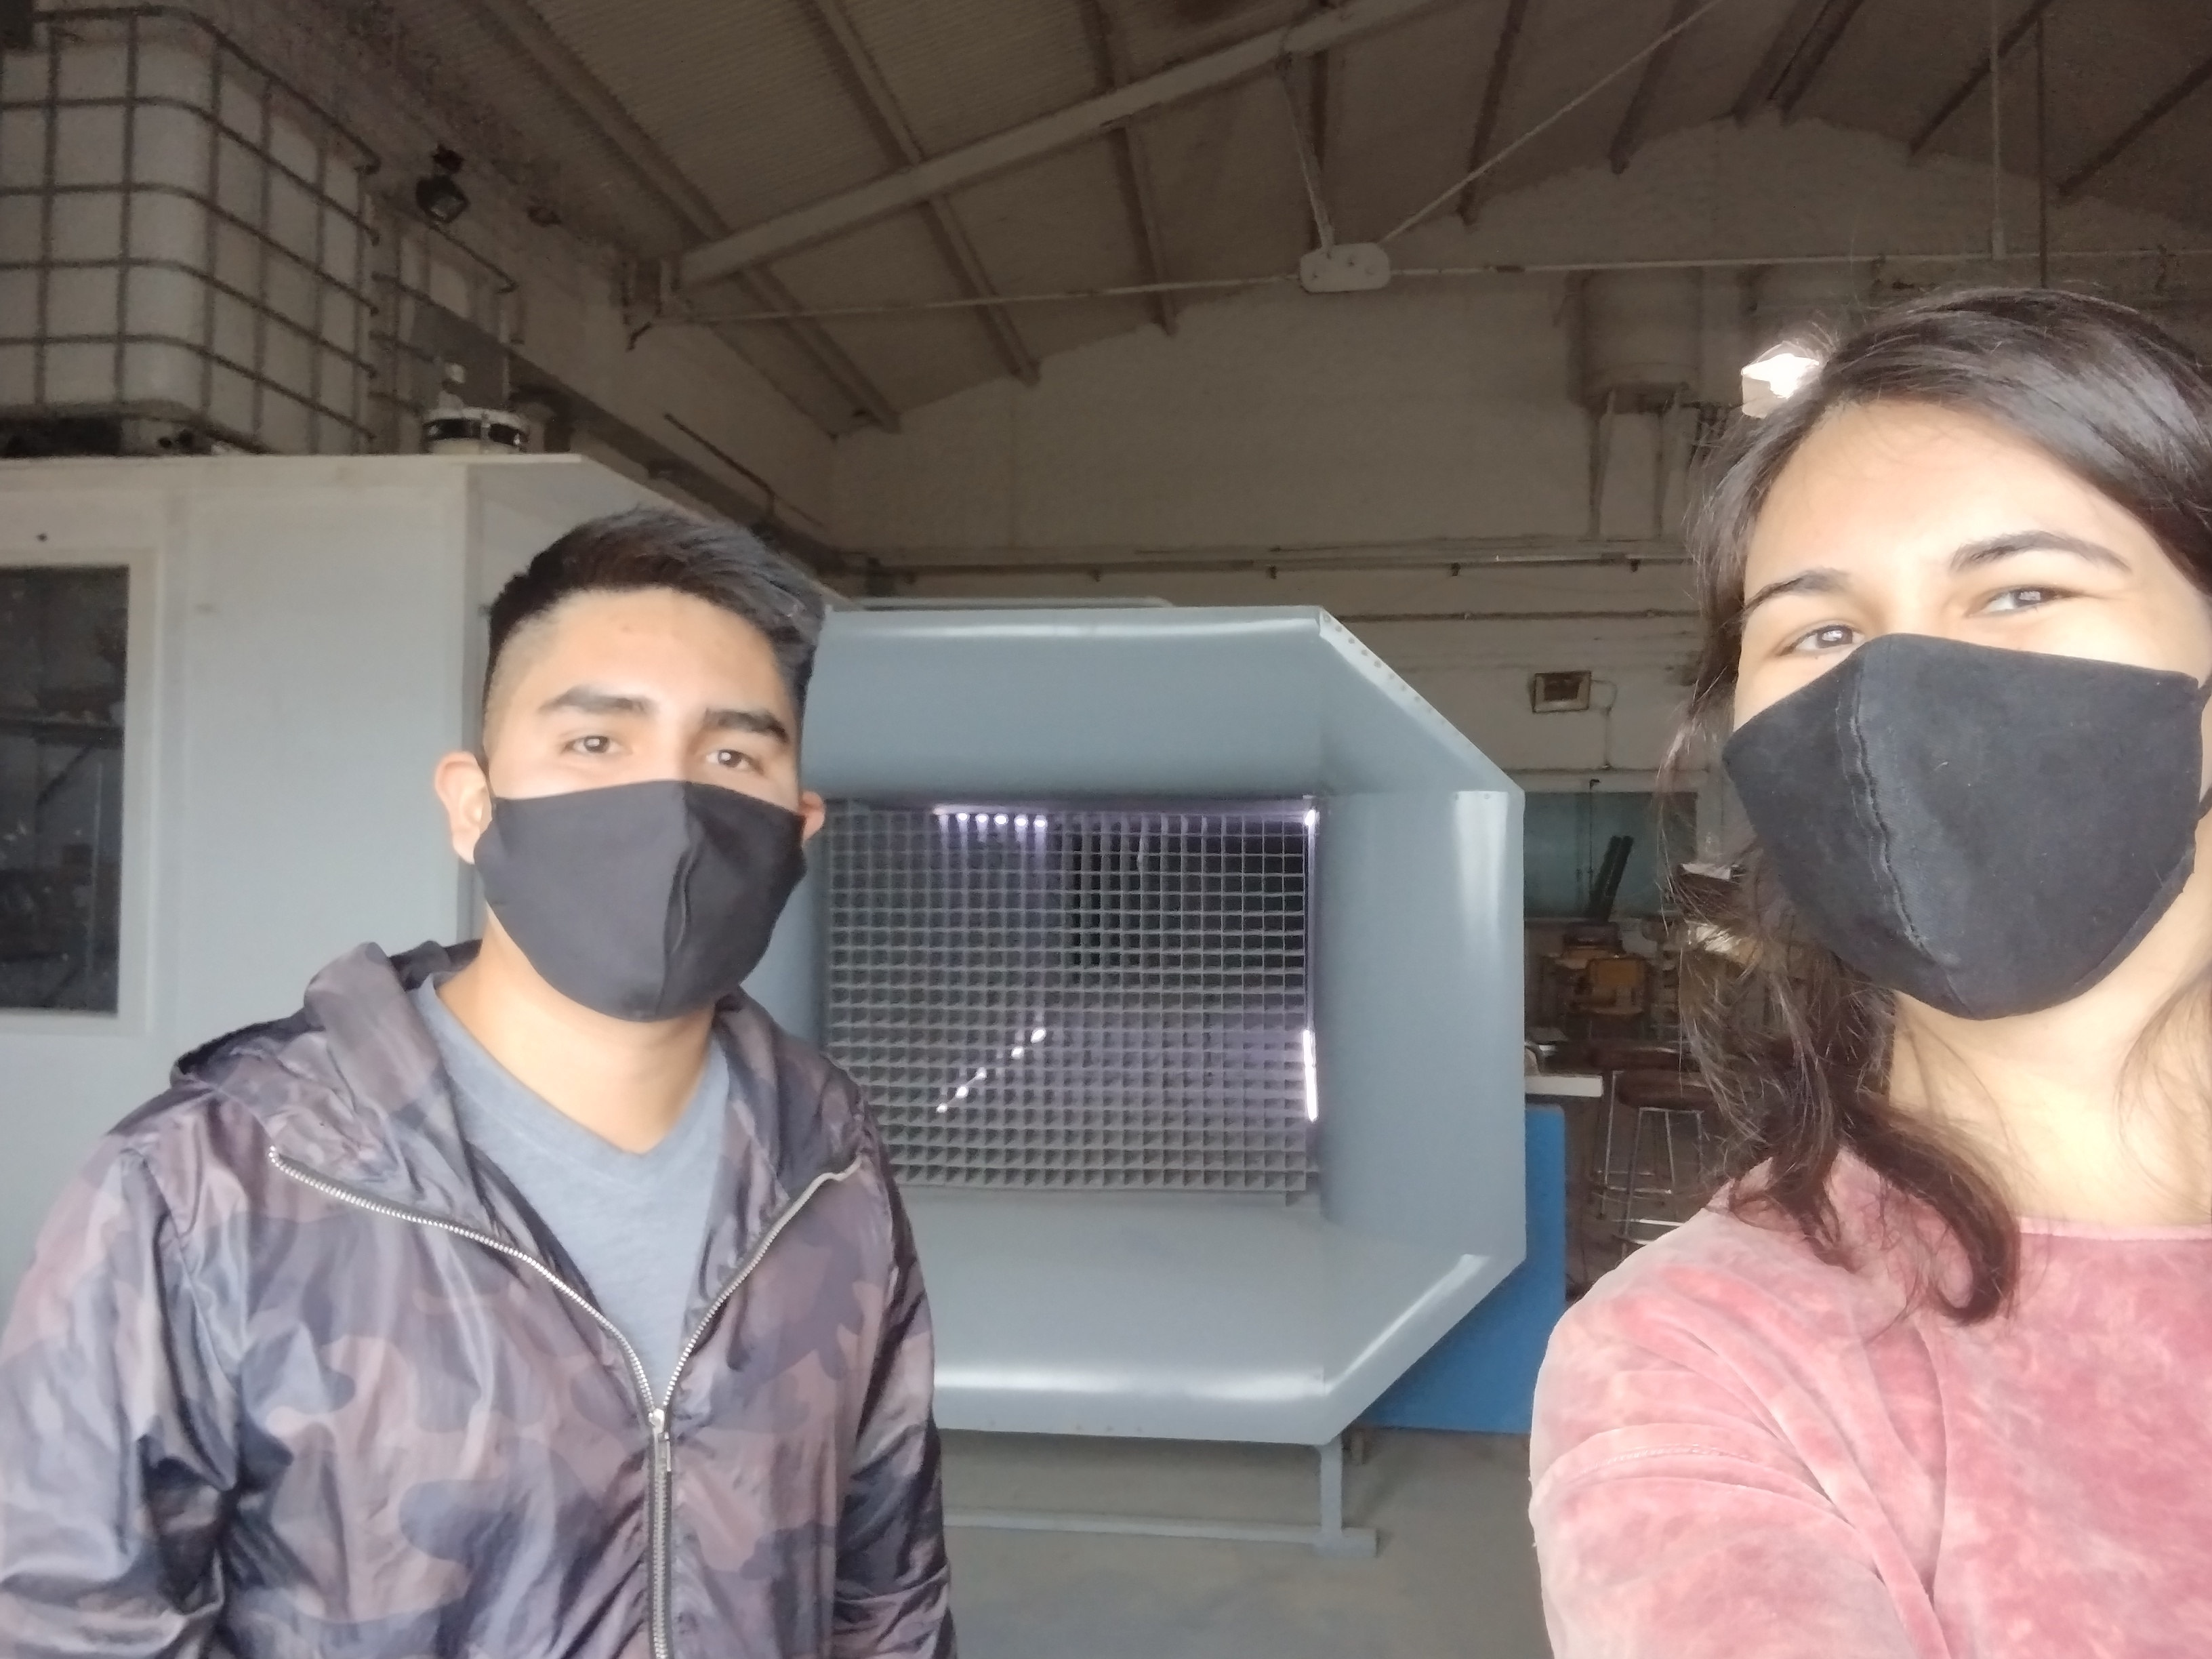
\includegraphics[scale=0.1]{corona.jpg}
	\captionof*{figure}{Autores al realizar el proyecto final de carrera en contexto de ``Pandemia'' por \textit{Covid-19}.}
	\label{fig:corona}
\end{figure}


\newpage

\newpage

	\tableofcontents
	\newpage
	\listoffigures
	\newpage
	\listoftables
	\newpage


	\section{Introducción}
	En el Laboratorio de Fluidos de la Universidad, se utiliza el Túnel de Viento para realizar el contraste de anemómetros y experimentos para distintas materias. Gran parte de estas aplicaciones requieren que se conozca la velocidad del fluido (aire). Por lo tanto, variación de presión, humedad, presión atmosférica y temperatura son variables requeridas para lograr estimarla con mayor precisión.
Cada variable debe ser medida de forma manual con sus respectivos instrumentos para luego ingresar estos valores a una tabla (generada de forma estadística) y obtener una estimación de la velocidad del fluido.\\

El túnel en sus comienzos, para realizar distintas mediciones, utilizaba un control de velocidad a lazo abierto en el que se modificaba la resistencia del motor, para cambiar la velocidad del aire en pasos discretos. Actualmente, desde principios del año 2020 se utiliza un variador de velocidad de la marca \textbf{Long Shenq}, con él se obtiene un control mas continuo en la frecuencia del motor. \\

Realizar este proceso de forma manual, se torna engorroso y poco práctico para la realización de varias mediciones por lo que se realiza este trabajo final de carrera para realizar la \textit{Automatización del Túnel de Viento de la UNPSJB}.

\newpage


	\section{Objetivo}
	El banco de pruebas cuenta con un punto de apoyo donde se conecta el motor y sus componentes mecánicos, ademas dentro de esta plataforma existe un sistema de medición que posee sensores, variador y PLC para poder realizar prácticas de laboratorio.
Un banco de pruebas puede ser un prototipo de gran desarrollo industrial o simplemente un banco formado para realizar pruebas educativas. \\

El objetivo de este trabajo final para la cátedra de Automatización Industrial es construir un banco de pruebas para ser utilizado por cualquier persona dentro el laboratorio de Automatización y Control. Se espera realizar uno que sea capaz de controlar la presión o caudal de agua a través de un sistema ideado y construido por nosotros, que cuente con:
\begin{itemize}
    \item Motor trifásico 1,5kW (Altium)\textit{-Proporcionado por la cátedra-}
    \item PLC (\textit{Schneider Electric} - M340) \textit{-Proporcionado por la cátedra-}
    \item Variador de velocidad (\textit{Schneider Electric}- ATV312 ) \textit{-Proporcionado por la cátedra-}
    \item Panel de control
        \subitem Botón de emergencia
        \subitem Encendido/ apagado
        \subitem Potenciómetro para variar velocidad
        \subitem Alarmas visuales
    \item HMI
        \subitem Control general del banco
        \subitem Información en tiempo real
        \subitem Histórico de datos
        \subitem Alarmas
\end{itemize}


\newpage

\section{Definiciones}
\begin{tcolorbox}[colback=blue!5!white,colframe=blue!75!black,title=Motor eléctrico]
	Los motores eléctricos son máquinas que transforman la energía eléctrica en energía mecánica a través de la generación de campos magnéticos.
\end{tcolorbox}

\begin{tcolorbox}[colback=blue!5!white,colframe=blue!75!black,title=Variador de velocidad]
	Es utilizado para controlar la velocidad de giro de un motor.
	Para regular las revoluciones, se debe tener en cuenta las características del motor, ya que este tiene una curva propia de funcionamiento. Un variador es capaz de generar elementos control de aceleración, frenado, seguridad, control de torque y operaciones que mejoran la eficiencia energética del motor.
\end{tcolorbox}

\begin{tcolorbox}[colback=blue!5!white,colframe=blue!75!black,title=PLC]
	Es una computadora que se utiliza en la ingeniería de automatización para controlar procesos en las industrias.
\end{tcolorbox}

\begin{tcolorbox}[colback=blue!5!white,colframe=blue!75!black,title=SoMove]
	Software que permite configurar variadores de velocidad pertenecientes a la empresa \textit{Schneider Electric}.
\end{tcolorbox}

\begin{tcolorbox}[colback=blue!5!white,colframe=blue!75!black,title=Unity Pro]
	Software común de programación, puesta a punto y
	explotación de los autómatas Modicon, M340, Premium, Quantum y
	coprocesadores Atrium de la empresa \textit{Schneider Electric}.
\end{tcolorbox}

\begin{tcolorbox}[colback=blue!5!white,colframe=blue!75!black,title=CANopen]
	CANopen es un protocolo con aplicación industrial de bajo nivel para aplicaciones de automatización. Conecta dispositivos entre sí mediante mensajes entre pares. Basado en el estándar de comunicaciones físicas CAN. Se utiliza en redes de comunicación tipo esclavo, multimaestro. 
\end{tcolorbox}

\begin{tcolorbox}[colback=blue!5!white,colframe=blue!75!black,title=ModBus]
	Modbus es un protocolo de comunicaciones utilizado para transmitir información a través de redes en serie entre dispositivos electrónicos, basado en la arquitectura maestro/esclavo o cliente/servidor, diseñado en 1979 por Modicon para su gama de PLC. Convertido en un protocolo de comunicaciones estándar en la industria. Además, esta red de comunicación industrial usa los protocolos RS232/RS485/RS422.
	%http://microelecblog.blogspot.com/2013/12/configuracion-atv312-para-red-modbus.html
\end{tcolorbox}

\begin{tcolorbox}[colback=blue!5!white,colframe=blue!75!black,title=HMI - SCADA]
	Ambas tecnologías, HMI y SCADA, son utilizadas en conjunto en la industria de la automatización. SCADA proporciona funciones de supervisión, alarmas y control, mientras que HMI proporciona las herramientas que necesita para desarrollar imágenes que los operadores pueden usar para monitorear su proceso.
\end{tcolorbox}

\begin{tcolorbox}[colback=blue!5!white,colframe=blue!75!black,title=iFIX]
	Software desarrollado por \textit{General Electric} donde se puede desarrollar aplicaciones sencillas típicas de HMI, o bien, aplicaciones SCADA más complejas como la gestión de elementos y distribución de alarmas.
\end{tcolorbox}
\newpage

	\section{Túnel Aerodinámico}
	
Un túnel de viento es una herramienta que puede tener dos fines hoy en día, ya sea para un uso recreativo o propósito científico.
Como uso científico se utiliza para observar los efectos del movimiento de aire al rededor de objetos sólidos, como tambien para la calibración de anemómetros.
\begin{figure}[htb]
	\centering
	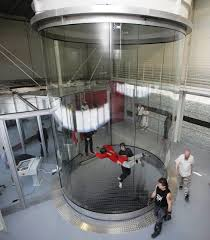
\includegraphics[scale=0.35]{tvert1.jpg}
	\caption{Tunel uso recreativo}
	\label{fig:tunelRec}
	\end{figure}
Los túneles de viento se pueden clasificar en túneles abiertos o cerrados y a su vez pueden ser verticales u horizontales.

\subsection{Historia del Túnel UNPSJB}
\footnote{http://www.ing.unp.edu.ar/mecanica/Paginas/Tunel.htm} 
	El túnel aerodinámico del Laboratorio de Mecánica de Fluidos (LMF) de la Facultad de Ingeniería de la Universidad Nacional de la Patagonia San Juan Bosco (UNPSJB) es un circuito abierto (tipo Eiffel) con cámara de ensayos cerrada. Puede clasificarse como un túnel “pequeño de baja velocidad”, con una longitud total de 11m, una velocidad máxima de 18 m/s y una cámara de ensayos con un área de 0,8m2.
	\\
	La entrada del túnel cuenta con canalizadores, comúnmente denominados "panal de abejas", que favorecen la formación de un flujo uniforme y homogéneo propiciando mejores resultados en los experimentos.
	\\
	La cámara de ensayos es vidriada para poder observar con claridad el flujo y está incorporada en un módulo extraíble del túnel, lo cual permite fácil acceso para el armado de los distintos objetos a ensayar.
	\\
	La variación de la velocidad del aire dentro de la cámara se consigue por dos vías: modificando la velocidad del motor para lograr una aproximación, y mediante la apertura de compuertas ubicadas entre el rodete y la zona de ensayo, para el ajuste fino. La toma aire desde el exterior a través de las compuertas actúa como by-pass, modificando el flujo principal del túnel y controlando su velocidad.
	\\
	Los distintos ensayos que se realizan en el túnel son:
	\\
	- Determinación de coeficientes de resistencia y sustentación de distintos cuerpos y perfiles aerodinámicos.
	- Determinación de distribución de presiones a través de diferentes objetos como perfiles aerodinámicos, edificios, puentes, automóviles, etc.
	- Visualización con humo del flujo a través de distintos obstáculos.
	- Estudio del comportamiento dinámico de generadores eólicos.
	- Calibración de anemómetros. 

	\begin{figure}[htb]
		\centering
		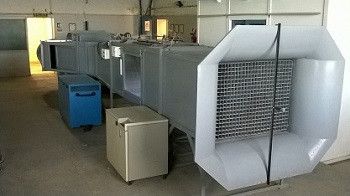
\includegraphics[scale=0.35]{tunel_unpsjb.JPG}
		\caption{Tunel UNPSJB}
		\label{fig:tunelUni}
		\end{figure}

		\subsubsection{Motor}
		
		\subsubsection{Vairador}

		\paragraph{¿Qué es y para que se utiliza?}
		\paragraph{Variador ----- modelo que tenemos}

		
	
\newpage
	\section{Fluido: Aire}
	\subsection{Ecuación velocidad del aire} \label{sec:ecvel}
	
		\begin{tcolorbox}[colback=blue!5!white,colframe=blue!75!black,title=I2C]
			Es un puerto y protocolo de comunicación serial, define la trama de datos y las conexiones físicas para transferir bits entre 2 dispositivos digitales. El puerto incluye dos cables de comunicación, SDA (Datos seriales) y SCL (reloj serial). Además el protocolo permite conectar hasta 127 dispositivos esclavos con esas dos líneas, con hasta velocidades de 100, 400 y 1000 kbits/s. \end{tcolorbox}
Para comenzar con las pruebas lo primero que se realizó es la conexión de diversos sensores en una protoboard. Se generó un programa de Arduino dónde a través de I2C se realizaba la comunicación. \\ Conjuntamente con estos sensores de Presión, Humedad y Temperatura se utilizó un sensor para medir presión diferencial, para digitalizar estos datos valores se utilizó un convertidor analógico digital.\\
Este primer prototipo se utilizó para comparar los datos de presión, temperatura y humedad con los valores obtenidos con los dispositivos calibrados con los que cuenta el laboratorio.
Como paso siguiente se eligieron los sensores con menos fluctuaciones y se armó una placa para que no se desconecten.
\\
Los elementos que se decidió utilizar fueron los siguientes:
\begin{itemize}
	\item  \textbf{BME280:} Sensor de presión atmosférica, temperatura y humedad relativa.
	\item \textbf{SI7021:} Sensor de temperatura y humedad relativa.
	\item \textbf{MPXV7002:} Sensor de presión diferencial.
	\item \textbf{ADS1115:} Convertidor analógico digital 16bits.
\end{itemize}	

\begin{figure}[htb]
	\centering
	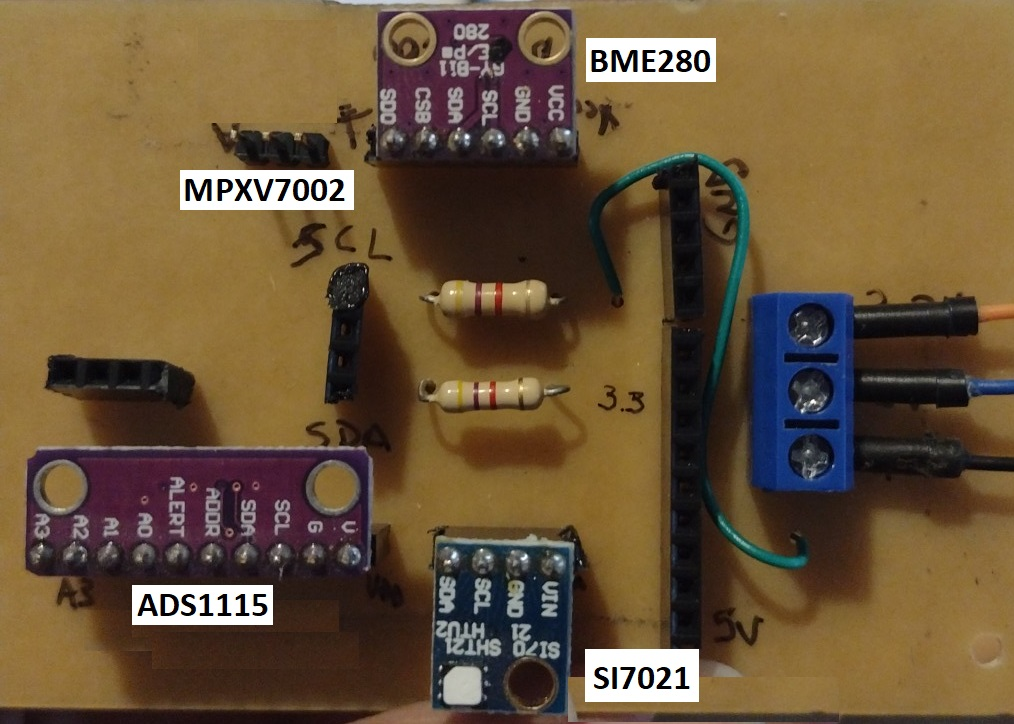
\includegraphics[scale=0.2]{sensores.jpg}
	\captionof{figure}{Placa con sensores}
	\label{fig:sensoresa}
\end{figure}

\subsection{Ecuación velocidad del aire}
El Laboratorio de Mecánica de Fluidos, antes de comenzar con este proyecto utilizó un archivo Excel para hacer la corrección de la velocidad del aire. En este se calcula matemáticamente la densidad del aire en función de la presión, temperatura y humedad atmosférica. Esta ecuación fue desarrollada dentro del programa de Arduino para observar como dato final la velocidad del aire.

	%	densidad_funcion_P_T_H.pdf  dentro del drive


    \subsection{Programa Arduino}
        \subsubsection{Ecuación velocidad del aire}
	%	densidad_funcion_P_T_H.pdf  dentro del drive
    \subsection{Pruebas}
    aca explicar que se hizo sin filtros y porq se filtro despues
        \subsubsection{Filtros}
        que filtro se utilizo y porq y cuando
    - Poner donde se agrego.

\newpage
	\newpage
	%\section{Desarrollo}
	\subsection{Lazo de corriente} \label{sec:lazoI}

Se realizó la modificación de los parámetros nombrados en la sección \ref{sec:error} y se corroboró que el error no aparecía nuevamente al cambiar el modo de funcionamiento del variador.

Para realizar la comunicación del microcontrolador con el variador de velocidad se decidió utilizar el modo de funcionamiento de entrada analógica de dos hilos (\textbf{Ai1}) ingresados por la bornera de la figura \ref{fig:born}. Este modo analógico puede ser configurado de 0-10V o 0-20mA a través del “jummper J3” (Figura \ref{fig:placals}).

Se optó por la utilización un lazo de corriente, este tiene ventajas sobre el lazo de tensión ya  que es más estable en largas distancias y más inmune a los ruidos eléctricos e interferencias electromagnéticas. Normalmente, se utilizan lazos de corriente de 4-20mA para poder observar si hubiera fallas en el circuito, por lo que fue necesario adaptar la señal generada por el $\mu$C para seguir el estándar.



\begin{figure}[h]
	\centering
	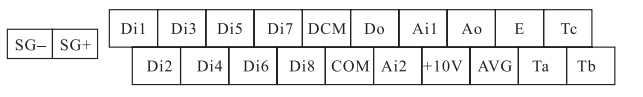
\includegraphics[width=0.7\linewidth]{imagenes/terminales.png}
	\caption{Terminales de control}
	\label{fig:born}
\end{figure}

\begin{figure}[htbp]
	\centering
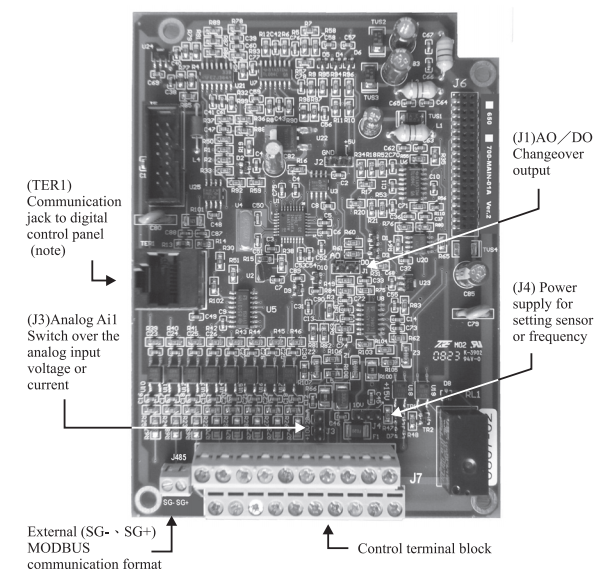
\includegraphics[width=0.7\linewidth]{imagenes/placa_ls}
\caption{Placa electrónica del variador de velocidad}
\label{fig:placals}
\end{figure}

La señal analógica para realizar el control del variador de velocidad fue generada por una señal PWM estipulada a través de la biblioteca \textit{TimerOne} del $\mu$C. Con esta biblioteca se configuró la frecuencia de la señal PWM, la cual fue de 25 kHz. 

Para la señal PWM generada, se utilizó el Pin 9 del $\mu$C, y se ajustó el ciclo de trabajo entre 0 y 1023 ya que era la resolución máxima que disponía la biblioteca. El Pin 9 de salida tiene un rango de tensión de 0 a 5V, por lo que fue necesario realizar la transformación de esta señal a una señal de corriente a través una “placa adaptadora de señal” (Figura \ref{fig:adapt}). Esta placa, tiene como entrada el valor de tensión anteriormente nombrado y genera una señal de salida de 0 a 20mA. Por medio de un parámetro del variador, se modificó la señal para adaptarla al estándar de 4 a 20mA.


\begin{figure}[htbp]
	\centering
	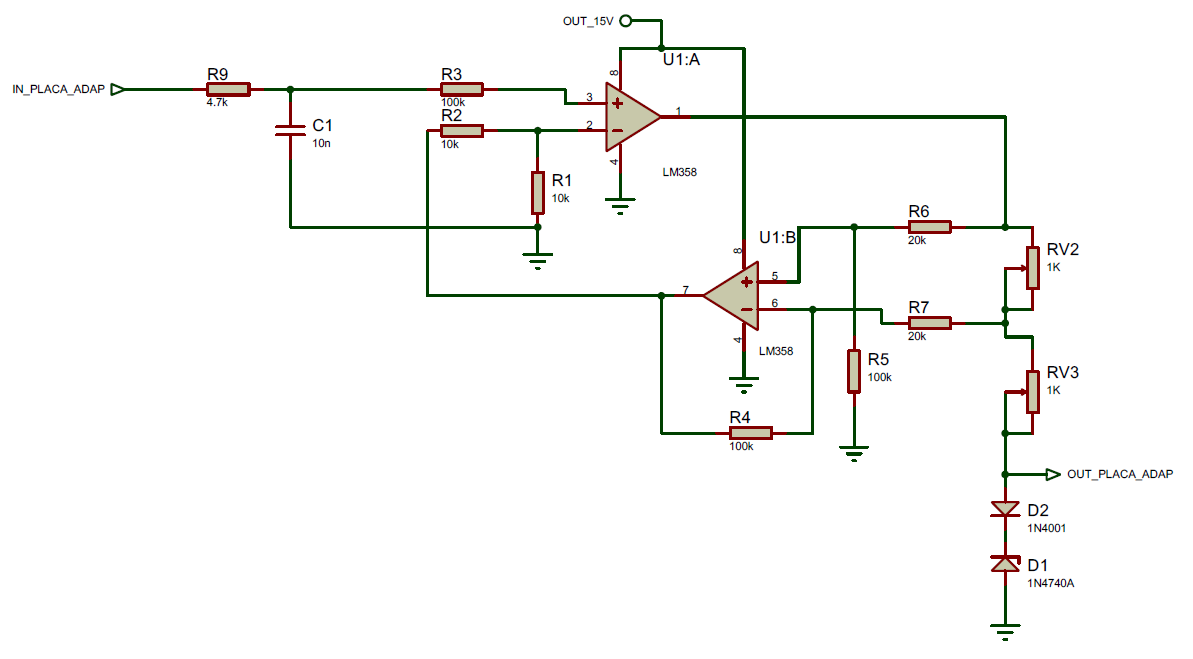
\includegraphics[scale=0.5]{adap_pl.png}
	\caption{Placa adaptadora de señal}
	\label{fig:adapt}
\end{figure}



\subsection{Estimación de la planta} \label{sec:estima}
    \subsubsection{Diagrama de trabajo}

Para realizar la estimación de la planta se muestra un diagrama de bloques del procedimiento que se siguió de forma resumida.

\begin{figure}[htb]
	\centering
	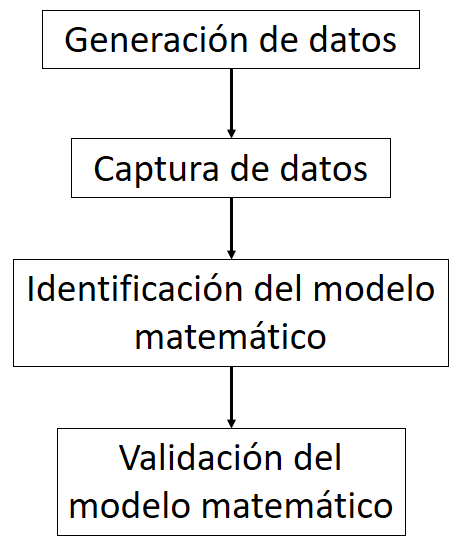
\includegraphics[scale=0.4]{planta_d.png}
	\captionof{figure}{Diagrama de bloques del procedimiento de modelado de la planta}
	\label{fig:planta_d}
\end{figure}

 \textbf{Generación de datos:} De acuerdo a diversas pruebas realizadas, se eligen las variables de mayor interés para analizarlas y asi poder enviar la información de forma eficaz.

 \textbf{Captura de datos:} A través del puerto serie y con Processing se realiza el almacenamiento de los datos de respuesta del sistema ante el estímulo de las señales de excitación. Posteriormente, el análisis de los datos y la generación de las gráficas correspondientes es realizado por medio de rutinas de código implementadas en Matlab.

 \textbf{Identificación del modelo matemático:} Se utilizaron varios métodos de identificación experimental, todos ellos analizados con la respuesta al escalón del sistema.

 \textbf{Validación del modelo matemático:} Una vez obtenida la mejor estimación, se efectuó una validación adicional a partir de la comparación de datos experimentales con los teóricos generados en simulaciones.






    \subsubsection{Método de estimación}

    Una vez que se determinó el valor de la ventana del filtro, velocidad de conmutación de PWM, tiempos de aceleración y desaceleración, etc, se utilizó el modo de ingreso de señal por lazo de corriente al variador de velocidad. 
    
    La Figura \ref{fig:bloques} muestra un diagrama resumido de los pasos a realizar para tomar datos de la planta. G(s) es el conjunto del túnel de viento, variador de velocidad y motor.


\begin{figure}[htbp]
	\centering
	\subfigure[Diagrama en bloques]{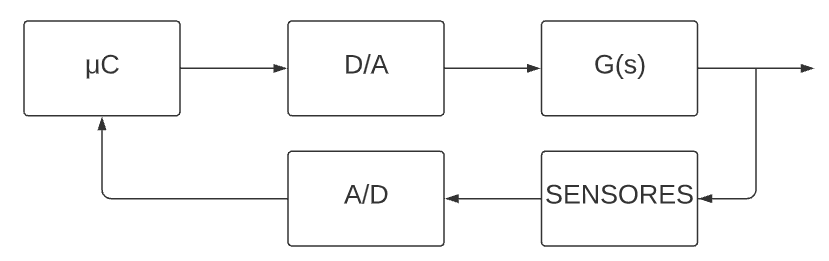
\includegraphics[scale=0.5]{bloques.png}}
	\centering
	\subfigure[Diagrama de conexión ]{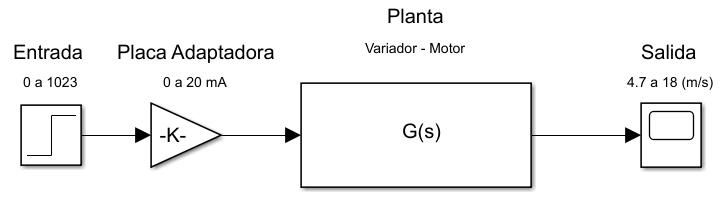
\includegraphics[scale=0.7]{Estimacion_1.png}} 
	\caption{Estimación de planta} \label{fig:bloques}
\end{figure}
 
    
    Para realizar la estimación de la planta se obtuvo y guardó tablas de datos con Processing, en las que se generó distintos escalones de entrada para la obtención de varias mediciones. En la figura \ref{fig:est2} se observa los valores de velocidad y los escalones que se realizaron durante una prueba generada para obtener los parámetros necesarios para la estimación de la planta.
    
    \begin{figure}[htb]
    	\centering
    	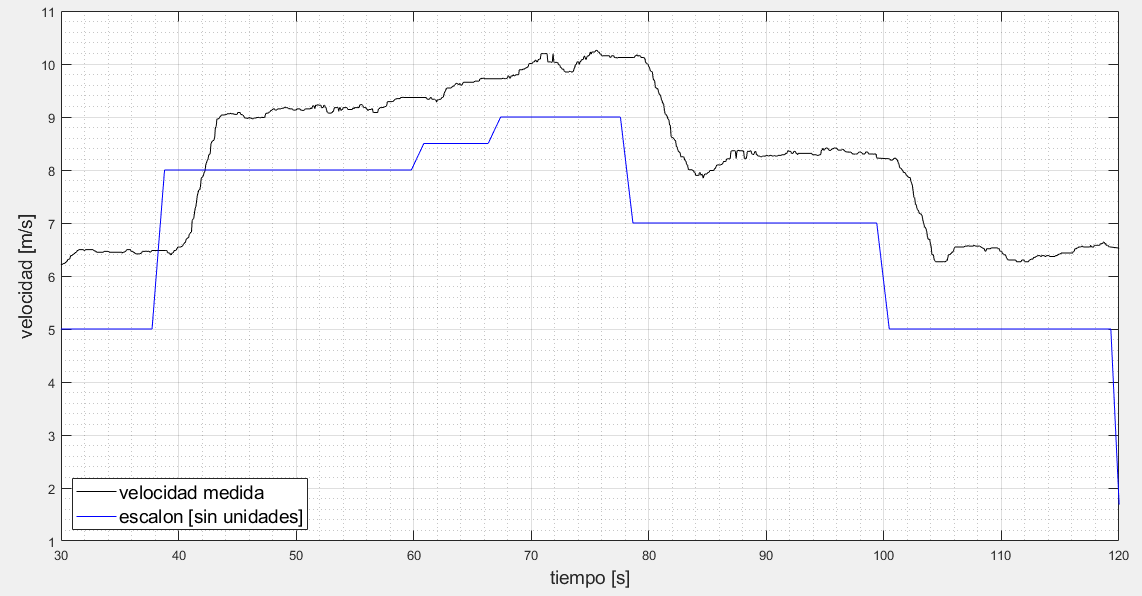
\includegraphics[scale=0.40]{estima.png} %pruba_1 del 0607
    	\captionof{figure}{Mediciones de velocidad a partir de distintos escalones dados}
    	\label{fig:est2}    
    \end{figure}
    
    Seguidamente, se procedió a generar un nuevo código de Matlab donde se cargó los datos obtenidos de la prueba (Figura \ref{fig:est2}) y con ellos se observaron las características necesarias de la figura (a) \ref{fig:pl2} para realizar la estimación de la planta a través de la comparación con la función de transferencia de un sistema de \textit{"2° orden con retardo"} \cite{pomares2011sistemas}.
    
    \begin{figure}[H]
    	\centering
    	\subfigure[Parámetros respuesta 2° orden]{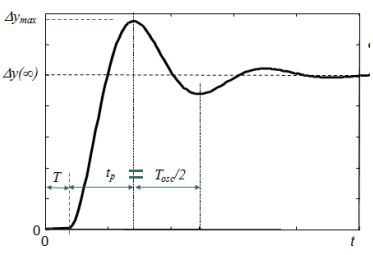
\includegraphics[scale=0.7]{parametros_seg.png}}
    	\subfigure[Estimación de parámetros]{\includegraphics[scale=0.35]{planta_seg1.png}} 
    	\caption{Estimación de planta} \label{fig:pl2}
    \end{figure}

El sistema de \textit{"2° orden con retardo"} posee la función de transferencia observada en la ecuación \ref{ec:G}.

 \begin{equation}
 	G(s)=\frac{k\omega_n^2}{s^2+2\xi\omega_ns+\omega_n^2}\ast e^{-T.s}
 	\label{ec:G}
 \end{equation}

La ecuación de sobre oscilación (Ecuación \ref{ec:amort}), es utilizada para calcular el factor de amortiguamiento ($\xi$)
\begin{equation}
	\delta\;=\;\frac{\triangle y_{max}-\triangle y\left(\infty\right)}{\triangle y\left(\infty\right)}=\;e\;^{-\frac{\xi\pi}{\sqrt{1-\xi^2}}}
	\label{ec:amort}
\end{equation}

La ecuación \ref{ec:tp} es utilizada para obtener el valor de la frecuencia natural ($\omega_n$) a partir del tiempo de pico.
\begin{equation}
t_p\;=\;\frac{T_{osc}}2\;=\;\frac\pi{\omega_n\sqrt{1-\xi^2}}
\label{ec:tp}
\end{equation}

    
    Con ayuda de un código generado en Matlab y ajustes manuales se llegó a la siguiente función de transferencia de segundo orden:
    
    \begin{equation}
    	\frac{Y(s)}{U(s)}=\frac{0,02483}{s^2+1,846s+1,535}*e^{-1.2.s}
    \end{equation}
   
    Esta función de transferencia se realizó para una entrada entre 0 y 1023, los cuales son el límite mínimo y máximo para determinar el ancho de pulso de la señal PWM como se ve en la sección \ref{sec:lazoI}.
    
    Para corroborar la elección de la planta se realizó en \textit{Simulink} la respuesta del sistema a los mismos escalones experimentales. En la figura \ref{fig:estim2} y \ref{fig:estim3}, se dispuso la respuesta experimental y la simulada para realizar la comparación.
    
    \begin{figure}[H]
    	\centering
    	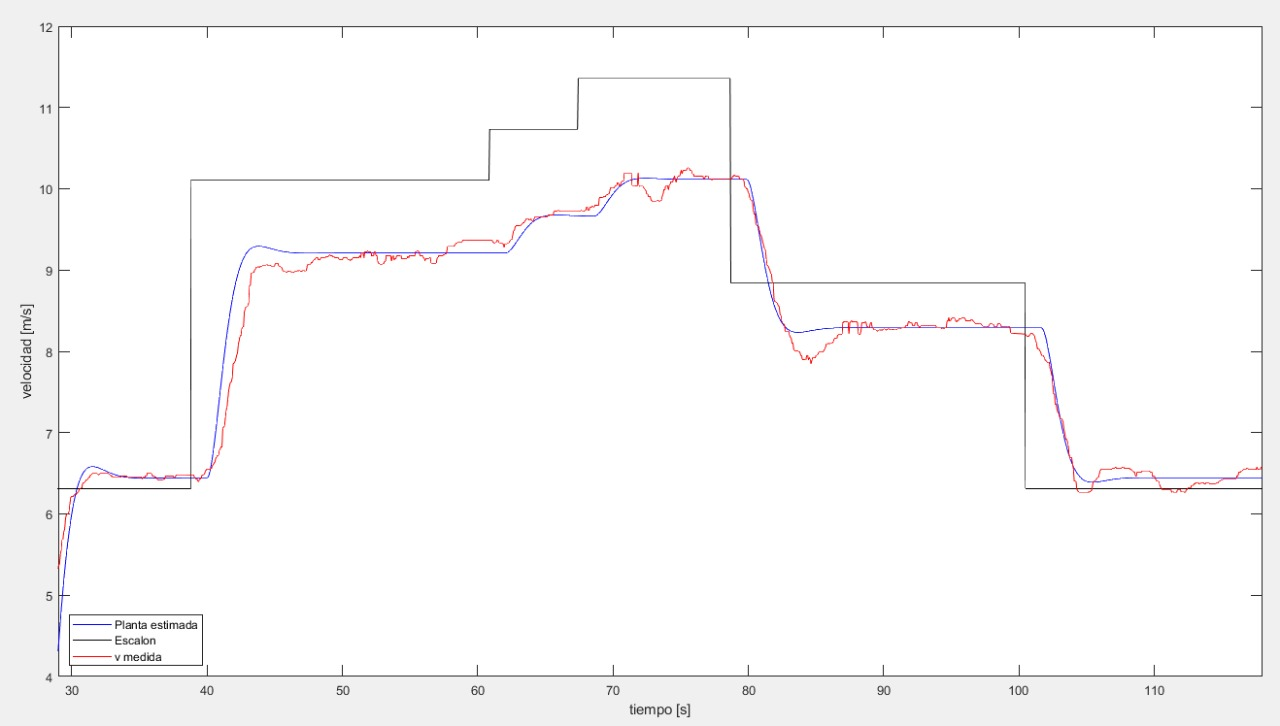
\includegraphics[scale=0.3]{estim2.jpeg}
    	\captionof{figure}{Corroboración de estimación de la planta. Ejemplo 1}
    	\label{fig:estim2}
    \end{figure}

\begin{figure}[H]
	\centering
	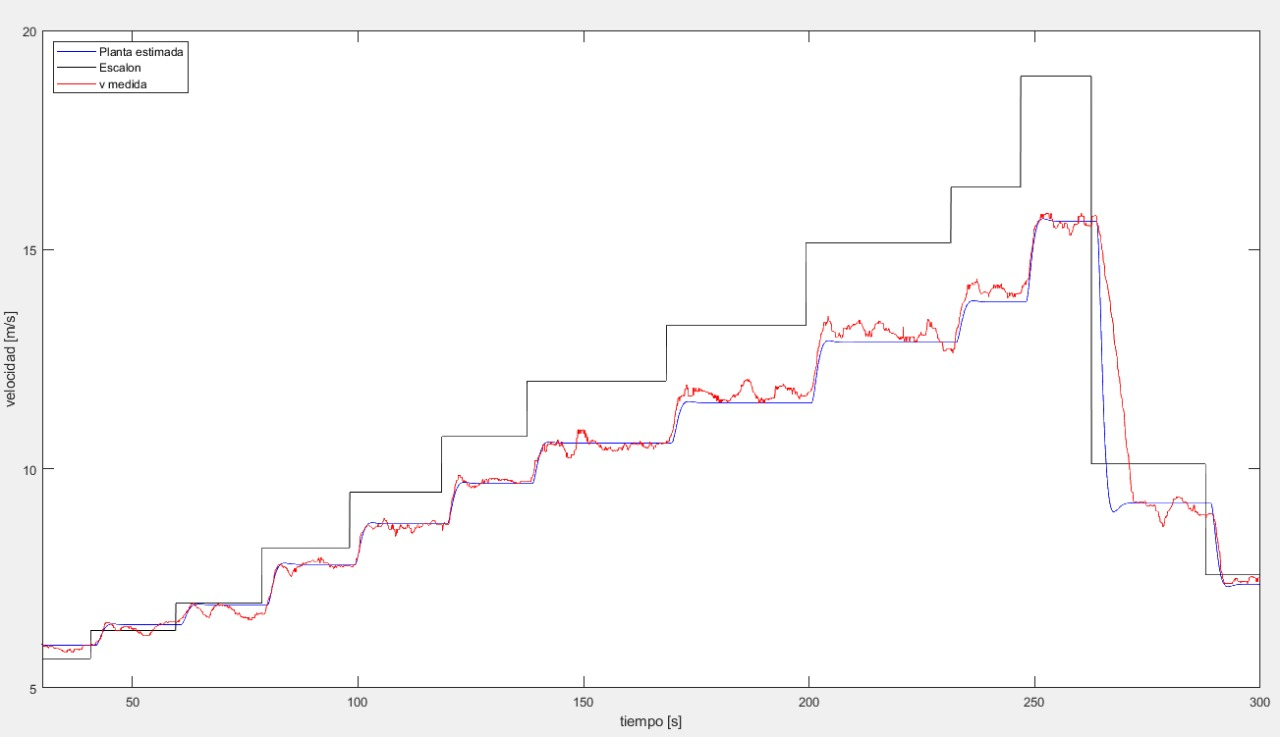
\includegraphics[scale=0.3]{estim3.jpeg}
	\captionof{figure}{Corroboración de estimación de la planta. Ejemplo 2}
	\label{fig:estim3}
\end{figure}
       
    \subsection{Control}
    Para el cálculo en primera instancia del controlador PID, se utilizó la herramienta de \textit{Matlab}, y a partir de los primeros valores se realizaron pequeñas modificaciones, todas con el formato PI (proporcional - integrador) hasta obtener varios tipos de respuesta.
    Con los distintos valores de PI (Tabla \ref{tab:pid}) se realizaron pruebas en el Túnel del viento con escalones en la velocidad de referencia de 6 - 7,5 - 8,5 - 7,5 - 7 - 6 m/s,  un total de 5 ensayos para los mismos estímulos de entrada. En la figura \ref{fig:Lazo_Control} se observa el lazo de control que se utilizó. 
   
    \begin{figure}[H]
   	\centering
   	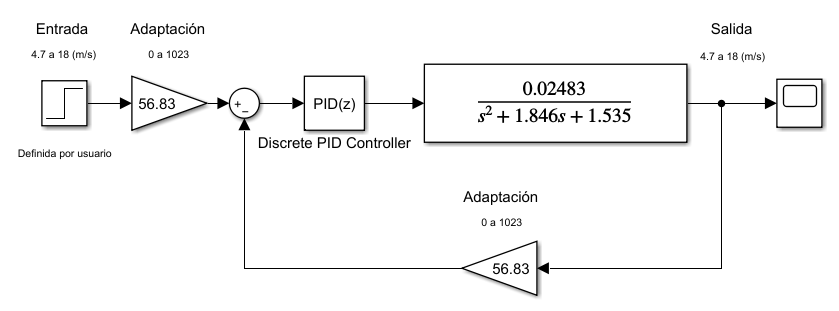
\includegraphics[scale=0.7]{Lazo_Control1.png}
   	\captionof{figure}{Lazo de control}
   	\label{fig:Lazo_Control}
   \end{figure}
    \begin{figure}[H]
    	\centering
    	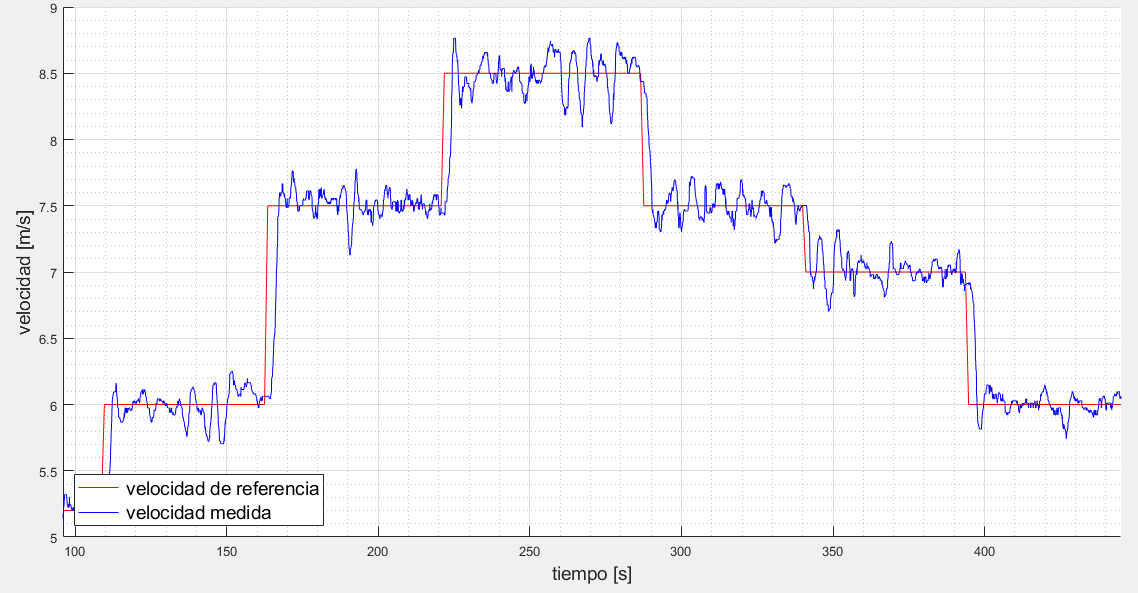
\includegraphics[scale=0.5]{pruebapid.png}
    	\captionof{figure}{Ejemplo de prueba realizada}
    	\label{fig:PI3}
    \end{figure}
    
    Los valores de cada configuración PI se muestran en la tabla siguiente
    \begin{table}[H]
    	\centering
    	\begin{tabular}{r|r|r|r|r|r|r|}
    		\cline{2-7}
    		\multicolumn{1}{l|}{} & \multicolumn{1}{c|}{\textbf{PI anterior}} & \multicolumn{1}{c|}{\textbf{Prueba3}} & \multicolumn{1}{c|}{\textbf{Prueba4}} & \multicolumn{1}{c|}{\textbf{Prueba5}} & \multicolumn{1}{c|}{\textbf{Prueba6}} & \multicolumn{1}{c|}{\textbf{Prueba7}} \\ \hline
    		\multicolumn{1}{|r|}{\textbf{P=}} & 0.225 & 0.0699 & 0.244 & 0.5451 & 0.6846 & 0.3286 \\ \hline
    		\multicolumn{1}{|r|}{\textbf{I=}} & 0.326 & 0.2035 & 0.2756 & 0.3599 & 0.4183 & 0.3107 \\ \hline
    	\end{tabular}
    \caption{Valores de PID's}
    \label{tab:pid}
    \end{table}
    
    Al visualizar las respuestas obtenidas por las diferentes configuraciones se puede realizar la comparación para un escalón en donde la velocidad sube (figura \ref{fig:pisubuda}) y otro donde la velocidad baja (figura \ref{fig:pibajada}).
    
    \begin{figure}[H]
    	\centering
    	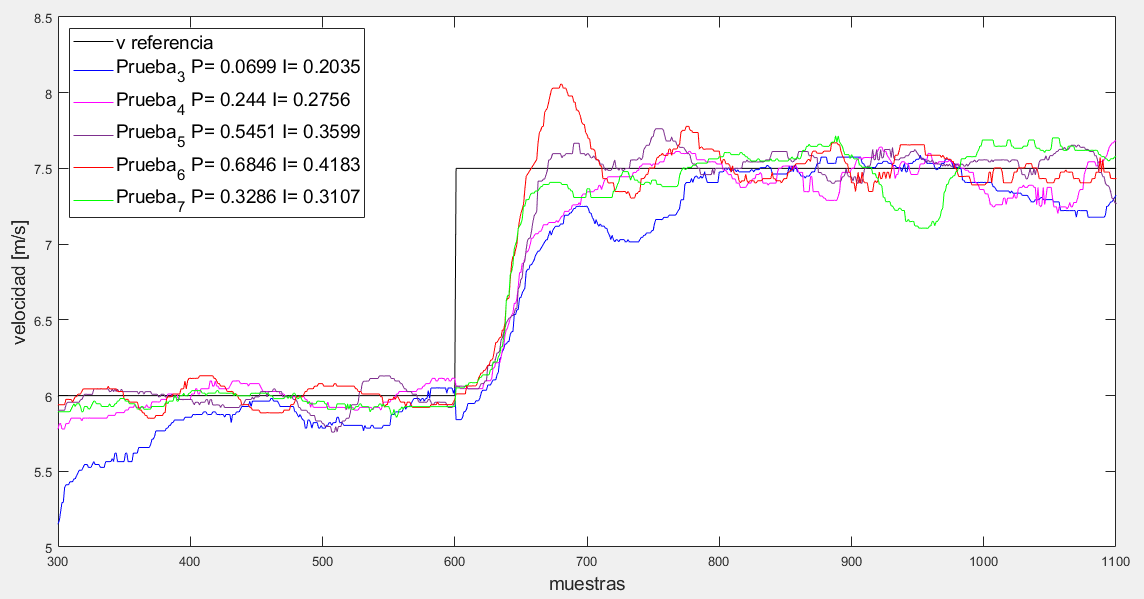
\includegraphics[scale=0.5]{pisubida.png}
    	\captionof{figure}{Comparación de PI, escalon de subida}
    	\label{fig:pisubuda}
    \end{figure}
    
    \begin{figure}[H]
    	\centering
    	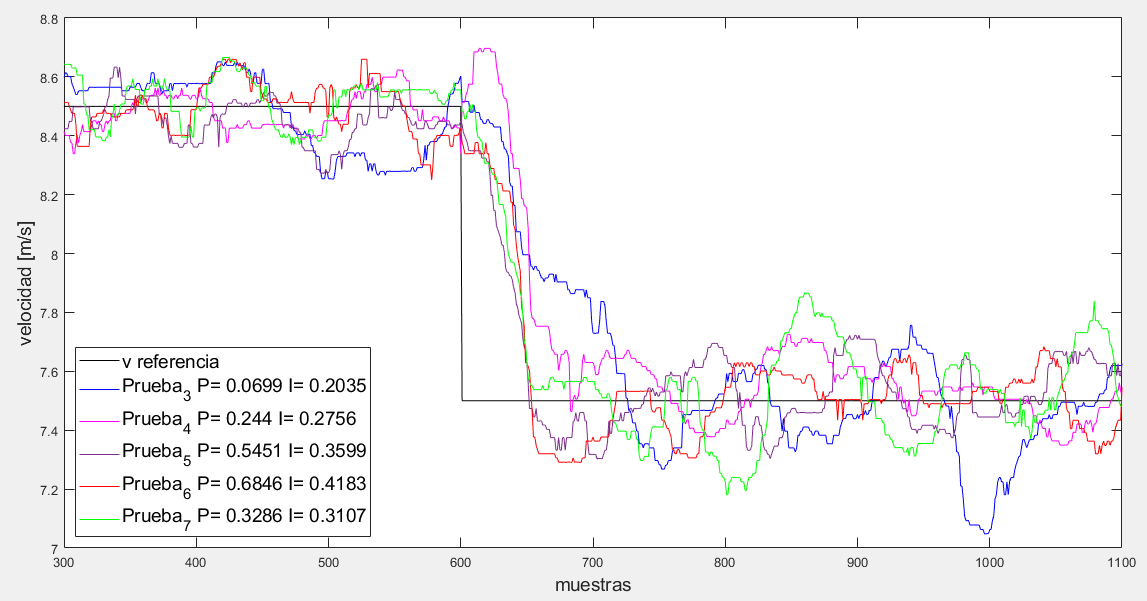
\includegraphics[scale=0.5]{pibajada.png}
    	\captionof{figure}{Comparación de PI, escalon de bajada}
    	\label{fig:pibajada}
    \end{figure}
    
    
    En la figura \ref{fig:mix} se pueden observar el sistema que genera mayor sobrepico, un sistema con una respuesta mas lenta, y un sistema con respuesta intermedia. 
    \begin{figure}[H]
    	\centering
    	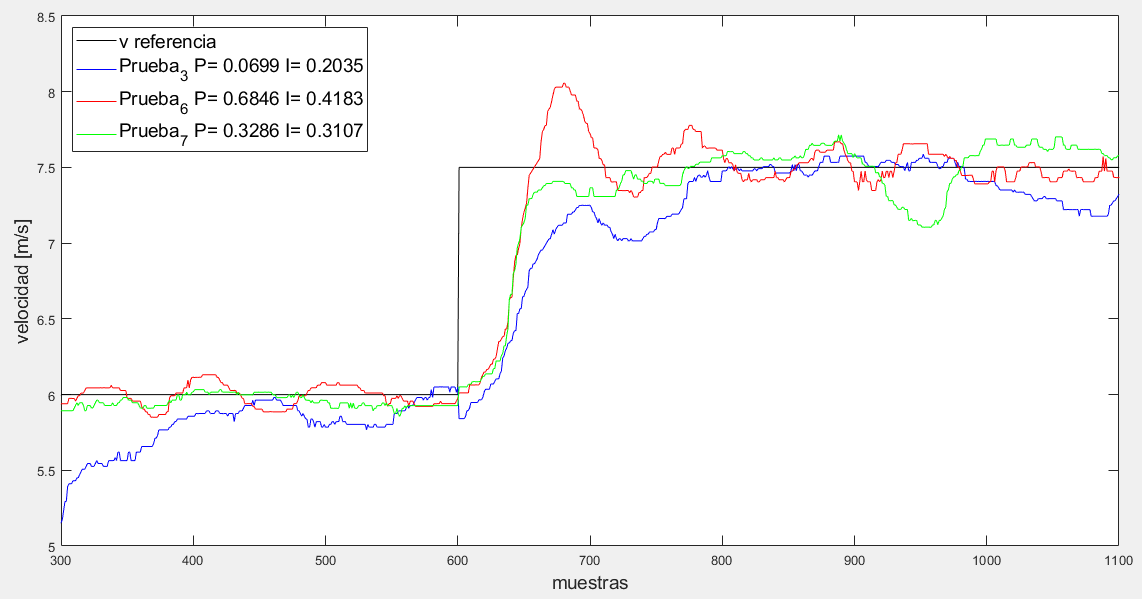
\includegraphics[scale=0.5]{mix.png}
    	\captionof{figure}{Comparación 3 sistemas PI}
    	\label{fig:mix}
    \end{figure}

	Al analizar los ensayos y obtener respuestas del sistema parecidas (Figura \ref{fig:Prueba_6} y \ref{fig:Prueba_7}) a las generadas en simulación, se determinó que la estimación de la planta se realizó de manera correcta, esto añadió mayor validez al sistema de simulación empleado en todas las pruebas. 
	
	\begin{figure}[H]
		\centering
		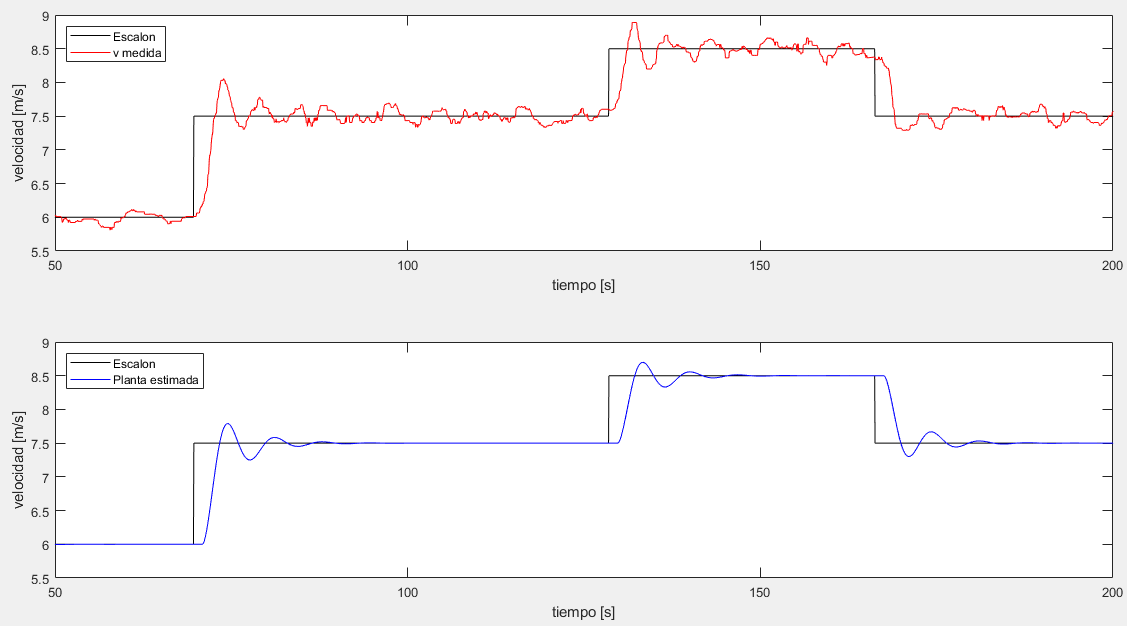
\includegraphics[scale=0.5]{Compa_Prueba6.png}
		\captionof{figure}{Datos Experimentales y Simulados para la \textit{Prueba6}}
		\label{fig:Prueba_6}
	\end{figure}   
\begin{figure}[H]
	\centering
	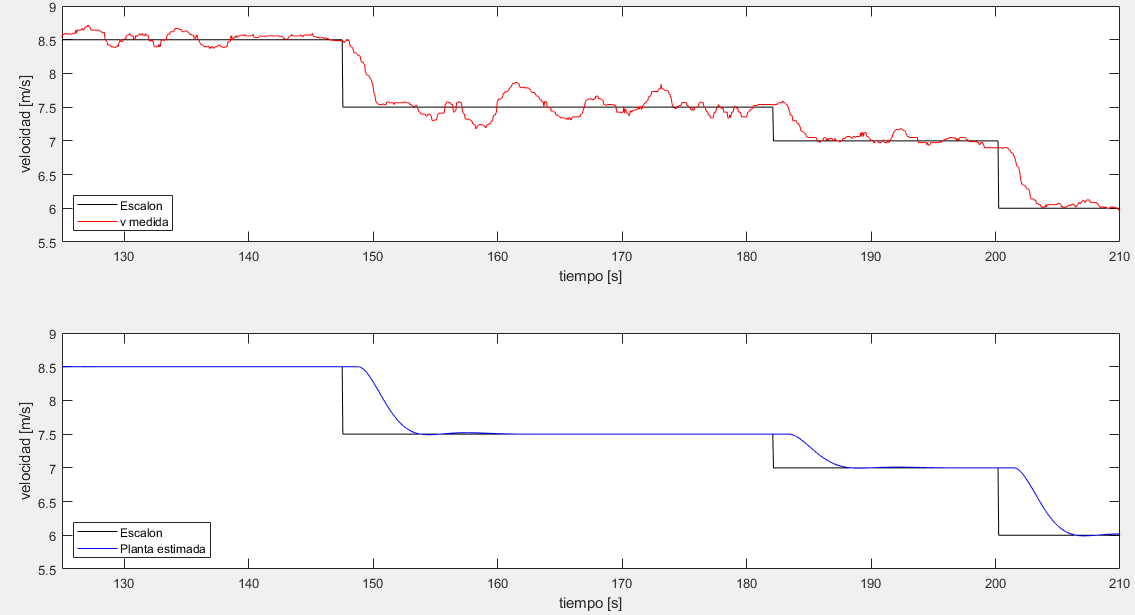
\includegraphics[scale=0.5]{Compa_Prueba7.png}
	\captionof{figure}{Datos Experimentales y Simulados para la \textit{Prueba7}}
	\label{fig:Prueba_7}
\end{figure}   
    \subsubsection{Implementación en $\mu$C}
    
    Para poder implementar en nuestro $\mu$C  el PID, se partió de la estructura interna o fórmula del controlador general discreto en el dominio Z (Ecuación \ref{PIDZ}) y se trabajó algebraicamente hasta llegar a una forma en donde aplicar la \textit{Transformada Inversa Z} sea más simple. Se utiliza esta herramienta matemática para llevar la ecuación del PID(z) al dominio de tiempo discreto.
    
     \begin{align}
    PID(z)\;=\frac{U(z)}{E(z)}&=\;P\;+\;I.T_s.\frac1{z-1}+D.\frac1{T_s}.\frac{z-1}z \label{PIDZ}\\
    \frac{U(z)}{E(z)}&=\;P\;.\frac{z^{-1}}{z^{-1}}+\;I.T_s.\frac1{z-1}.\frac{z^{-1}}{z^{-1}}+D.\frac1{T_s}.\frac{z-1}z.\frac{z^{-1}}{z^{-1}}\;\\
    \frac{U(z)}{E(z)}&=\;P\;+\;I.T_s.\frac{z^{-1}}{1-z^{-1}}+D.\frac1{T_s}.(1-z^{-1})\\
    \frac{U(z)}{E(z)}&=\frac1{1-z^{-1}}\left[P.\left(1-z^{-1}\right)\;+\;I.T_s.z^{-1}+\frac D{T_s}.(1-z^{-1})^2\right]\;\\
    U(z).\left(1-z^{-1}\right)&=E(z)\left[P+\;\frac D{T_s}+\left(\;I.T_s-P-2.\frac D{T_s}\right).z^{-1}+\frac D{T_s}.z^{-2}\right]\;\label{hola}
    \end{align}
Y si aplicamos la transformada inversa Z a la ecuación \ref{hola}:
\begin{align}
	u(k)\;=\;u(k-1)\;+\;\left(P+\frac D{T_s}\right).e(k)\;+\left(I.T_s-P-2.\frac D{T_s}\right).e(k-1)+\frac D{T_s}.e(k-2)\label{ecdiscreta}
\end{align}

De esta forma obtenemos la ecuación del PID en función de la muestra actual y anteriores, que nos sirve para implementar de manera directa en el $\mu$C. 

\subsubsection{Pruebas de control}
Para observar la respuesta del control se generó perturbaciones con las compuertas laterales del túnel (Figura \ref{fig:comp}), antes utilizadas para realizar variaciones de velocidad \cite{barila1993desarrollo} cuando el laboratorio no poseía un control continuo de ella porque se utilizaba un reóstato (8 posiciones) para modificar la resistencia rotórica del motor (Figura \ref{fig:reos}). 

\begin{figure}[H]
	\centering
	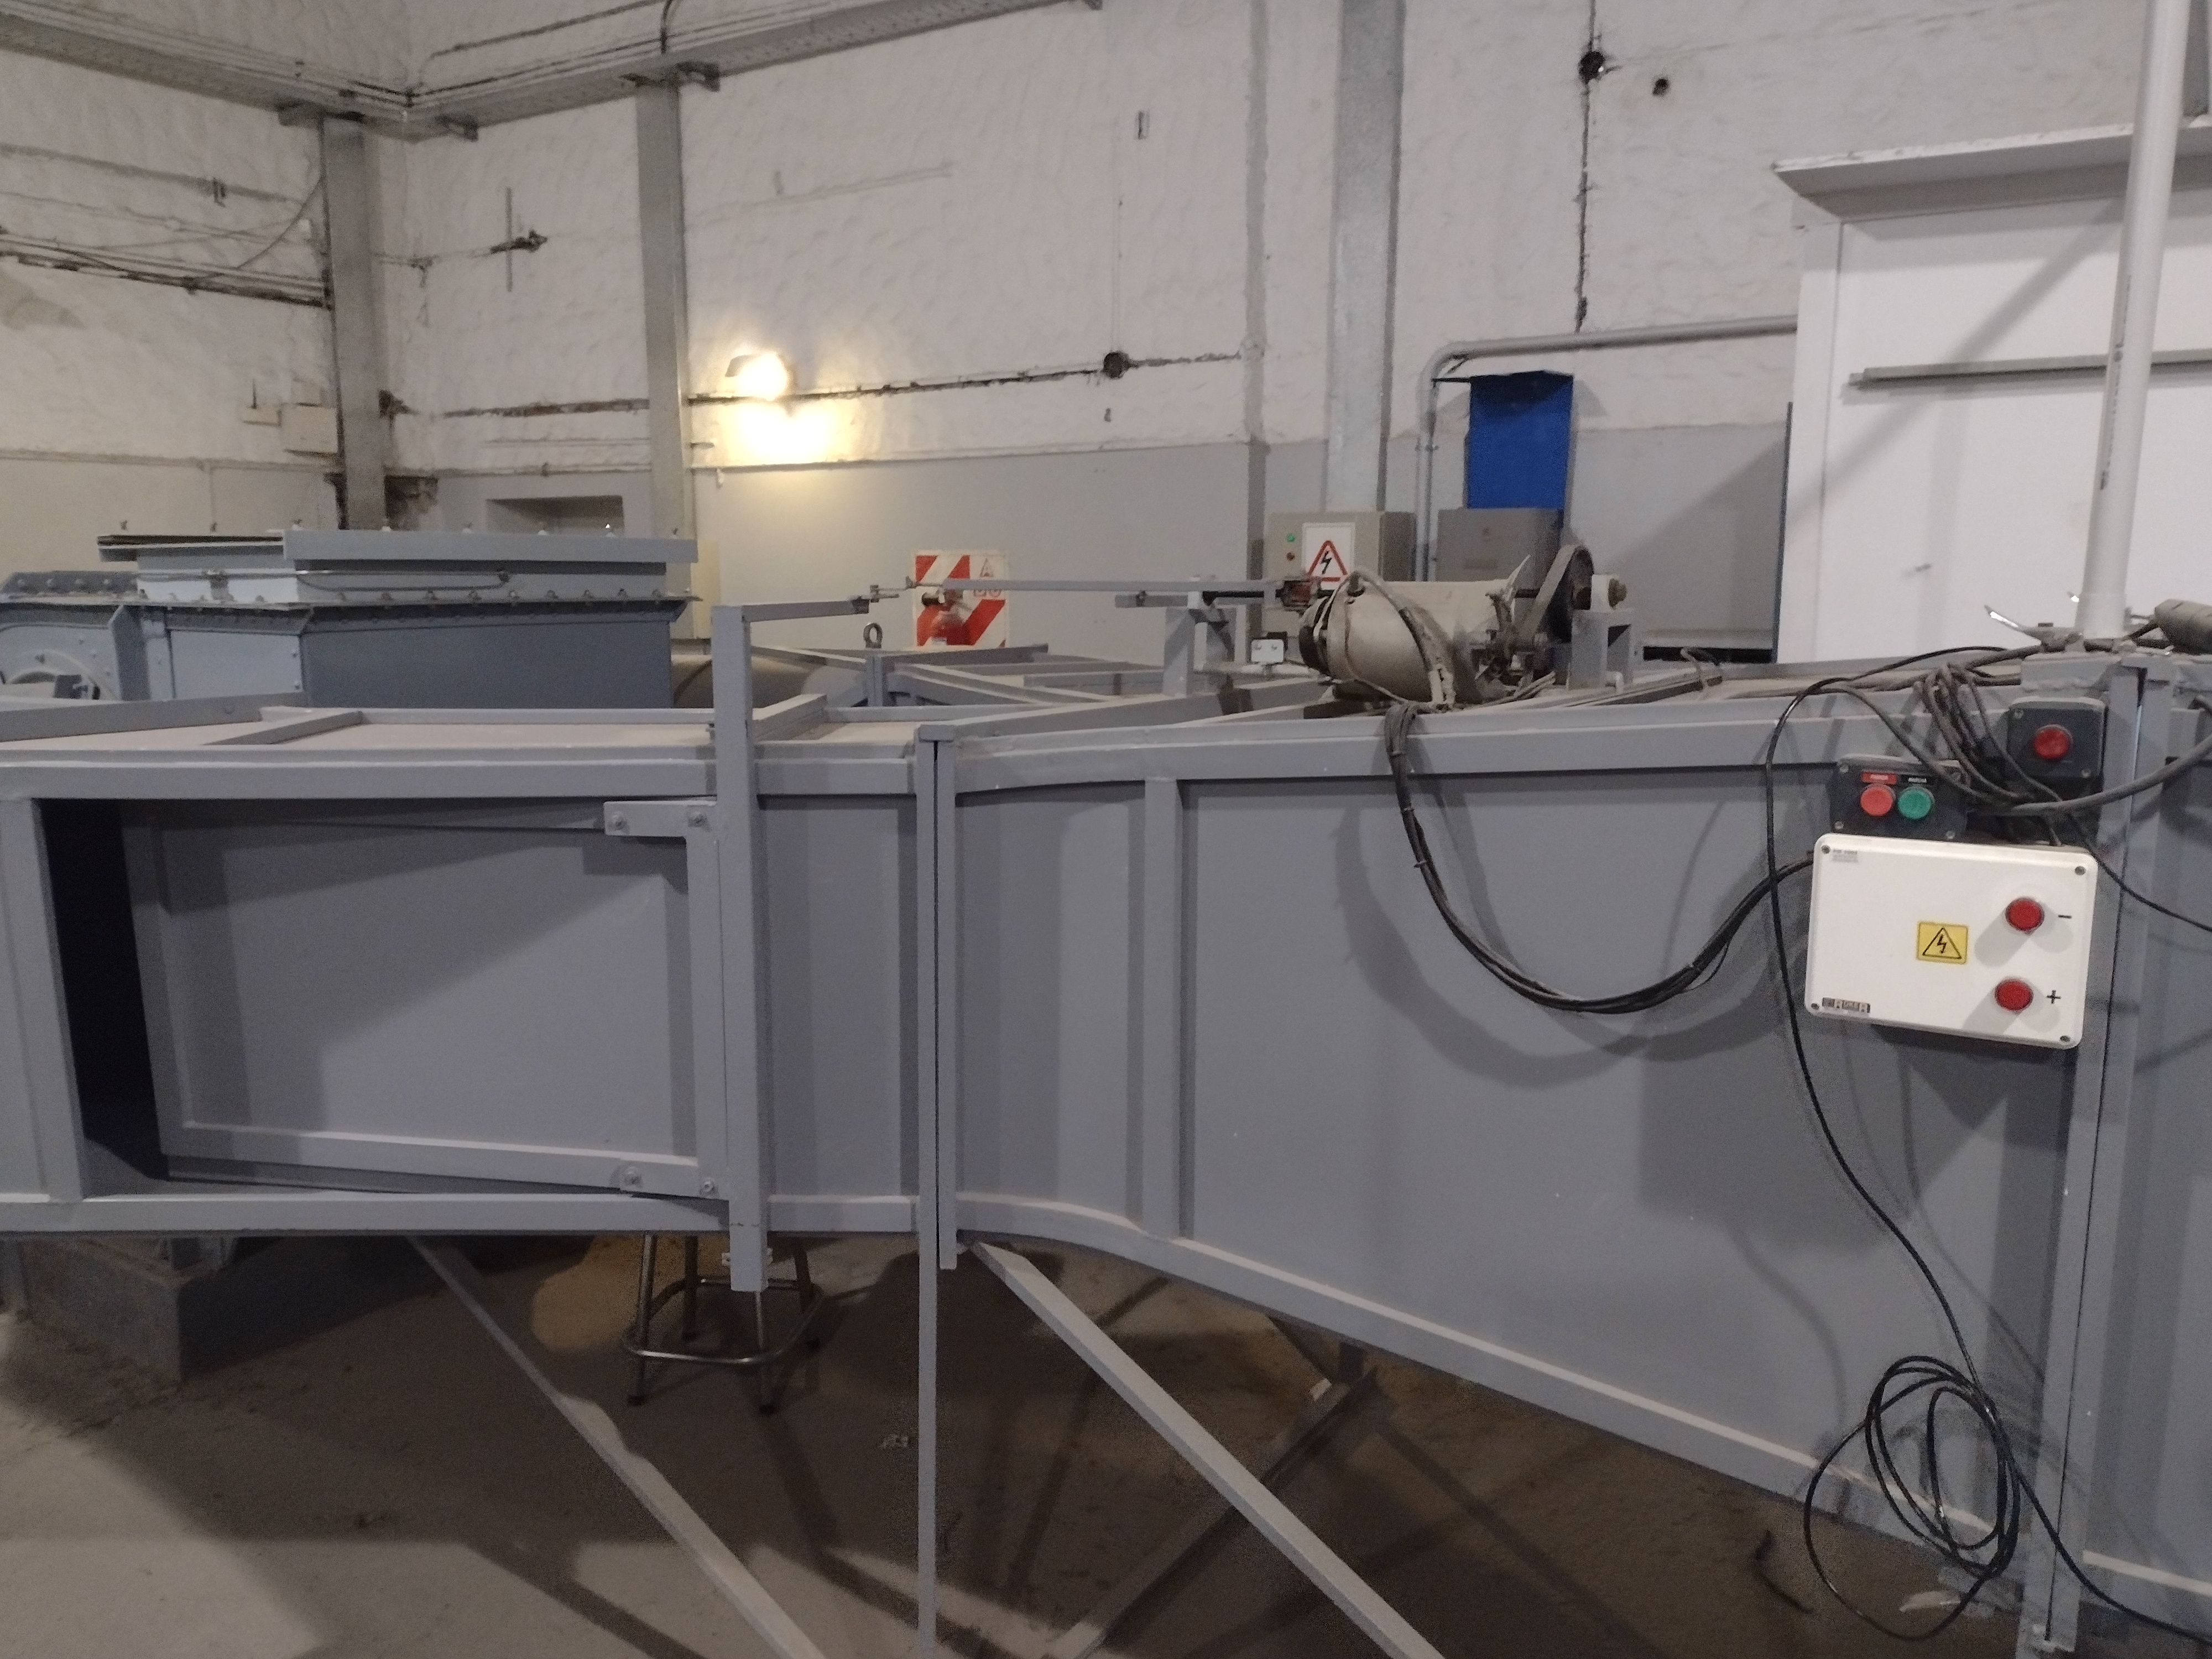
\includegraphics[scale=0.08]{comp.jpg}
	\captionof{figure}{Compuertas utilizadas como perturbaciones}
	\label{fig:comp}
\end{figure}

\begin{figure}[H]
	\centering
	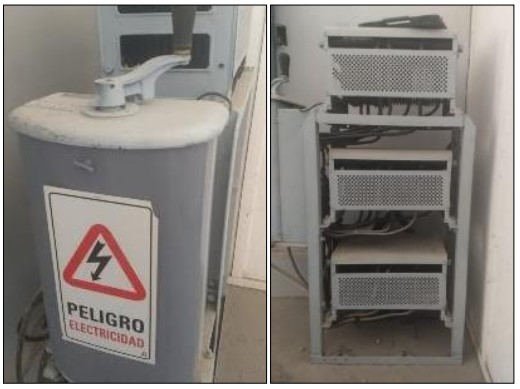
\includegraphics[scale=0.7]{reos.jpg}
	\captionof{figure}{Fotos del reóstato (izquierda) y del banco de resistencias (derecha)}
	\label{fig:reos}
\end{figure}

Para realizar estas pruebas de funcionamiento primero se encendió el túnel, se comenzó a guardar valores y se controló la velocidad del aire en 6 $m/s$, luego de unos segundos de funcionamiento se procedió a abrir las compuertas con el panel que se ve del lado derecho de la figura \ref{fig:comp}. Esta entrada de aire producía variaciones en la velocidad que el control implementado corregía según el PID utilizado. Se realizó pruebas donde se abrió y cerró las compuertas para observar estos cambios y el correcto control de velocidad (Figura \ref{fig:comp1} y \ref{fig:comp2}).


\begin{figure}[H]
	\centering
	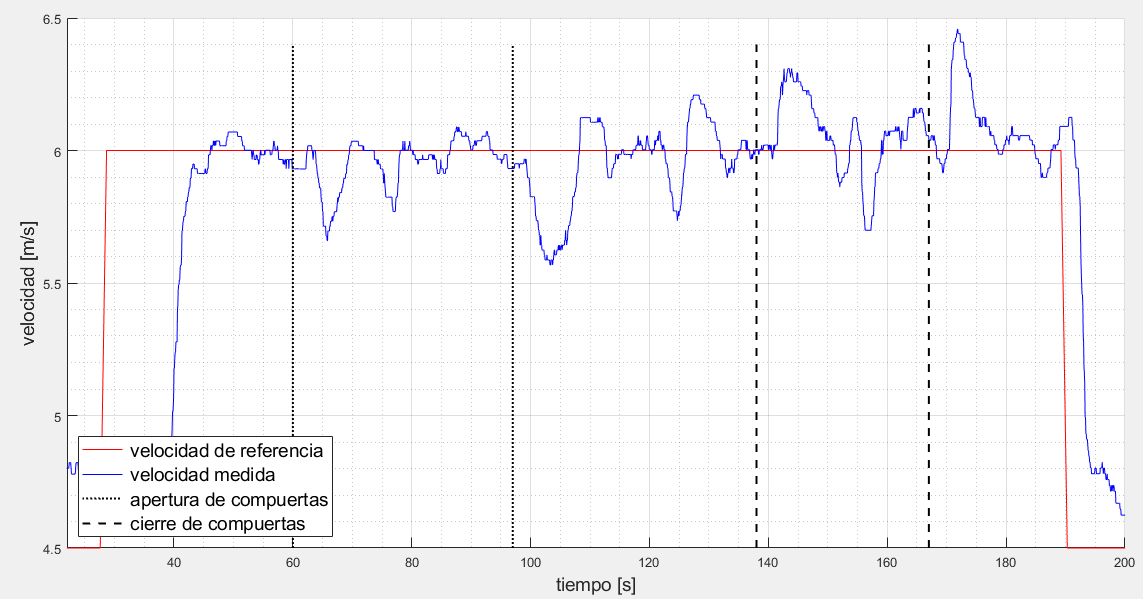
\includegraphics[scale=0.5]{compu1.png}
	\captionof{figure}{Comportamiento del sistema ante perturbaciones. Ejemplo 1.}
	\label{fig:comp1}
	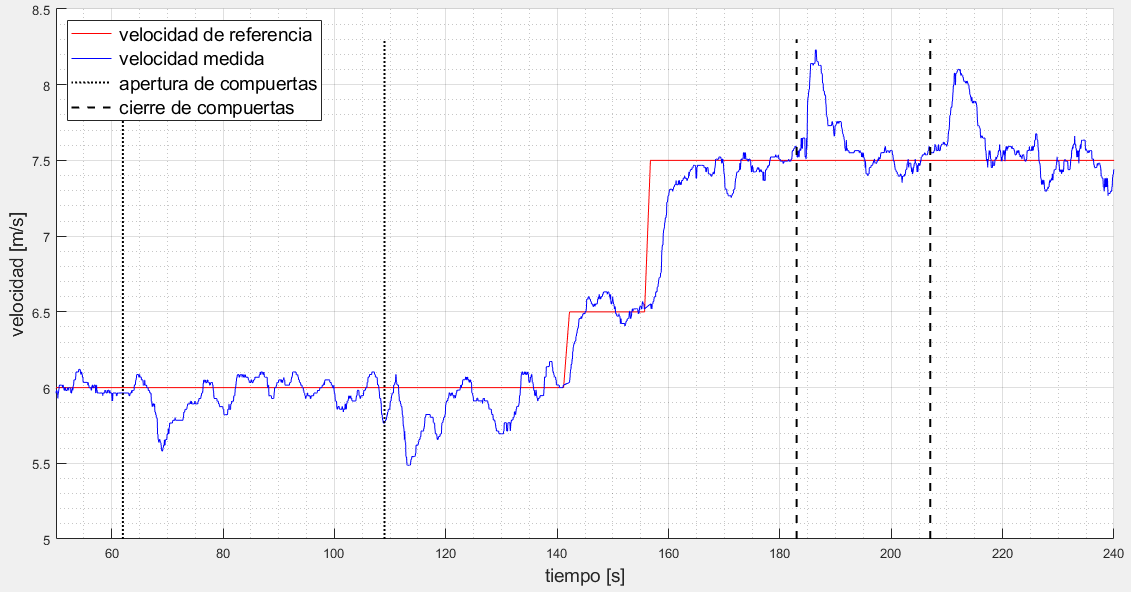
\includegraphics[scale=0.5]{comp2.png}
	\captionof{figure}{Comportamiento del sistema ante perturbaciones. Ejemplo 2.}
	\label{fig:comp2}
\end{figure}



    \newpage
	\newpage
	\section{Pruebas realizadas}
	\subsection{Comparación de densidades} \label{cap:densidades}

Una vez que se tuvo seguridad con los sensores elegidos se procedió a realizar una placa con estos elementos para que no se desconecten y produzcan errores como solía suceder mientras estaban en la protoboard (Figura \ref{fig:sensoresa}). \\
\begin{figure}[H]
	\centering
	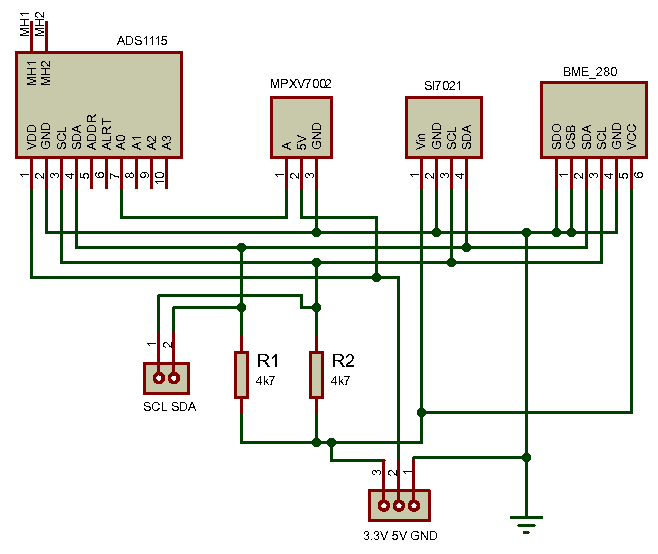
\includegraphics[scale=0.9]{placa_sensores.pdf}
	\captionof{figure}{Esquema de placa con sensores utilizados}
	\label{fig:sensoresa}
\end{figure}

A raíz de los resultados de varias mediciones, realizadas durante distintos días, y al realizar el contraste con el instrumento \textbf{TESTO 435} se decidió retirar de la caja los sensores de temperatura y humedad para que luego el cálculo de la velocidad del aire no esté afectado por posibles cambios de estos, ya que esta caja utilizada generaba un ambiente distinto al real dentro del laboratorio. Al colocar el sensor del lado externo, se realizaron tomas de valores en distintos momentos. Con ambos conjuntos de datos se procedió a obtener los valores de la densidad calculados con la fórmula \ref{ec_den}. Estos datos están expresados en la tabla \ref{densicalc}. 


\begin{table}[b]
	\centering
	\begin{tabular}{ll|l|l|l|l|l|l|l|l|l|}
		\cline{3-11}
		\multicolumn{2}{c}{} & \multicolumn{2}{|c|}{\textbf{T [$^{\circ}$$C$]}} & \multicolumn{2}{c|}{\textbf{H [$\%$] }} & \multicolumn{2}{c|}{\textbf{P [$Pa$]}} &  \multicolumn{2}{c|}{\textbf{\begin{tabular}[c]{@{}c@{}}Dens. calculada\\ {[}$kg/m^3${]}\end{tabular}}} & \multicolumn{1}{c|}{\multirow{2}{*}{\textbf{$e_r$ [$\%$]}}} \\ \cline{1-10}
		\multicolumn{1}{|c|}{\textbf{Fecha}} & \multicolumn{1}{c|}{\textbf{Obs.}} & \multicolumn{1}{c|}{\textbf{I}} & \multicolumn{1}{c|}{\textbf{S}} & \multicolumn{1}{c|}{\textbf{I}} & \multicolumn{1}{c|}{\textbf{S}} & \multicolumn{1}{c|}{\textbf{I}} & \multicolumn{1}{c|}{\textbf{S}} & \multicolumn{1}{c|}{\textbf{I}} & \multicolumn{1}{c|}{\textbf{S}} & \multicolumn{1}{c|}{} \\ \hline
		\multicolumn{1}{|l|}{29-abr} & interior & 19,4 & 19,3 & 43,5 & 38,5 & 100400 & 100450 & 1,1916 & 1,1931 & 0,128 \\ \hline
		\multicolumn{1}{|l|}{14-may} & interior & 16,1 & 18,4 & 54,6 & 43,5 & 101590 & 101570 & 1,2195 & 1,2099 & 0,781 \\ \hline
		\multicolumn{1}{|l|}{14-may} & interior & 16,5 & 18,9 & 53,7 & 42,5 & 101559 & 101559 & 1,2173 & 1,2077 & 0,794 \\ \hline
		\multicolumn{1}{|l|}{17-jun} & exterior & 15,2 & 15,5 & 54,3 & 48,6 & 103100 & 103090 & 1,2418 & 1,2404 & 0,109 \\ \hline
		\multicolumn{1}{|l|}{17-jun} & exterior & 13,8 & 15,1 & 59,2 & 52,4 & 102970 & 102910 & 1,2463 & 1,2397 & 0,527 \\ \hline
		\multicolumn{1}{|l|}{07-jul} & interior & 17,6 & 18,8 & 43,3 & 34,8 & 100260 & 100261 & 1,1978 & 1,1933 & 0,375 \\ \hline
	\end{tabular}
	\caption{Comparación de densidades calculadas}
	\label{densicalc}
\end{table}




Referencias de la tabla:
\begin{itemize}
	\item \textbf{I}: Instrumentos- Datos obtenidos con los instrumentos del Laboratorio de fluidos.
	\item \textbf{S}: Sensores- Datos obtenidos a partir de la medición con los sensores utilizados en el proyecto.
	\item \textbf{interior}- Mientras se realizaron las mediciones el sensor SH21 se encontraba dentro de la caja dónde estaba el Arduino y la placa reguladora.
	\item \textbf{exterior}- Las mediciones se realizaron con el sensor SH21 en el lado exterior sin que fuera afectado por el calentamiento de la placa reguladora.
\end{itemize}


Al tomar como valor verdadero los valores de THP medidos con los instrumentos calibrados, se puede observar que el error relativo del cálculo de densidad es menor al 1\%.


%C:\Users\glori\Desktop\DANIELA\VISUAL_DANI\Proyecto_Final_Tunel\Pruebas22.03.21

\subsection{Estimación de la densidad ante cambios de Temperatura y Humedad}
Notamos conveniente realizar la comparación de las densidades calculadas ante las variaciones que se tenían de humedad y temperatura respecto a los datos tomados por los elementos calibrados. En la tabla \ref{densTH} se observa en las celdas internas los valores calculados de densidad para humedad de 38$\%$ y 40$\%$ y temperatura 19$^{\circ}$C y 21$^{\circ}$C, estos datos fueron elegidos al observar las máximas variaciones de los datos tomados con el sensor \textit{SH21} y el instrumento \textit{Testo 435}, al mantener la presión atmosférica constante.
(Los valores con fondo gris corresponden a la diferencia de densidades).

\begin{table}[H]
	\centering
	\begin{tabular}{ll|l|l|l|} 
		\cline{3-4}
		&                                    & \multicolumn{2}{c|}{\textbf{Temperatura}}                                                       & \multicolumn{1}{l}{}                            \\ 
		\cline{3-4}
		&                                    & \multicolumn{1}{c|}{\textbf{19°C}}             & \multicolumn{1}{c|}{\textbf{21°C}}             & \multicolumn{1}{c}{\textbf{}}                   \\ 
		\hline
		\multicolumn{1}{|c|}{\multirow{2}{*}{\textbf{Humedad}}} & \multicolumn{1}{r|}{\textbf{38\%}} & 1,1945758                                      & 1,1859383                                      & {\cellcolor[rgb]{0.816,0.816,0.816}}-0,0086376  \\ 
		\hhline{|~----|}
		\multicolumn{1}{|c|}{}                                  & \multicolumn{1}{r|}{\textbf{40\%}} & 1,1943783                                      & 1,1857162                                      & {\cellcolor[rgb]{0.816,0.816,0.816}}-0,0086621  \\ 
		\hline
		& \multicolumn{1}{c|}{\textbf{}}     & {\cellcolor[rgb]{0.816,0.816,0.816}}-0,0001976 & {\cellcolor[rgb]{0.816,0.816,0.816}}-0,0002221 & \multicolumn{1}{l}{}                            \\
		\hhline{~~--~}
	\end{tabular}
	\caption{Cálculo de la densidad ante cambios de temperatura y humedad}
	\label{densTH}
\end{table}

Si se calcula la velocidad del aire con la formula \ref{ec_aire} en conjunto con los datos de la tabla \ref{densTH} y se utiliza una diferencia de presión constante de 32$Pa$ se puede observar que la diferencias de velocidades son inferiores a 0,03m/s (tabla \ref{velTH}) ante un cambio de dos grados de temperatura por lo que no se ve necesario realizar una corrección de valores.


\begin{table}[H]
	\centering
	\begin{tabular}{ll|l|l|l|} 
		\cline{3-4}
		&                                    & \multicolumn{2}{c|}{\textbf{Temperatura}}                                                     & \multicolumn{1}{l}{}                           \\ 
		\cline{3-4}
		&                                    & \multicolumn{1}{c|}{\textbf{19°C}}            & \multicolumn{1}{c|}{\textbf{21°C}}            & \multicolumn{1}{c}{\textbf{}}                  \\ 
		\hline
		\multicolumn{1}{|c|}{\multirow{2}{*}{\textbf{Humedad}}} & \multicolumn{1}{r|}{\textbf{38\%}} & 7,3195288                                     & 7,3461357                                     & {\cellcolor[rgb]{0.816,0.816,0.816}}0,0266068  \\ 
		\hhline{|~----|}
		\multicolumn{1}{|c|}{}                                  & \multicolumn{1}{r|}{\textbf{40\%}} & 7,3201342                                     & 7,3468236                                     & {\cellcolor[rgb]{0.816,0.816,0.816}}0,0266894  \\ 
		\hline
		& \multicolumn{1}{c|}{\textbf{}}     & {\cellcolor[rgb]{0.816,0.816,0.816}}0,0006054 & {\cellcolor[rgb]{0.816,0.816,0.816}}0,0006879 & \multicolumn{1}{l}{}                           \\
		\hhline{~~--~}
	\end{tabular}
	\caption{Cálculo de velocidad del aire ante cambios de temperatura y humedad}
	\label{velTH}
\end{table}

\subsection{Contrastación de diferencia de presión}

El sensor \textit{MPX7002} tiene como salida una tensión proporcional a la diferencia de presión medida, por lo que fue necesario utilizar un \textit{ADS1115} para transformar estos valores, a través de una constante, en datos de presión digitalizados. (Sección \ref{sec:ads1115}).

Para realizar un contraste del valor de presión diferencial producido por la velocidad del aire dentro del túnel, en el tubo Pitot, se procedió a realizar mediciones con el instrumento calibrado \textit{AXD 650}. Al poseer fluctuaciones anteriormente mencionadas, debidas al flujo turbulento, y dado que el AXD650 no posee salida de datos (solo por display), se filmaron el instrumento y los datos obtenidos por nuestro sistema, para poder, con posterioridad, ver la correlación entre ambos. Los dos videos se unieron y se realizaron diversas pausas para tomar al mismo tiempo ambos valores leídos. Como resultado se obtuvo la tabla \ref{difpres}, luego se generó un gráfico de puntos con las muestras tomadas y se observó que el error es mayor para diferencias de presión mayores a 100 Pa (Figura \ref{fig:condifpres}).

\begin{figure}[H]
	\centering
	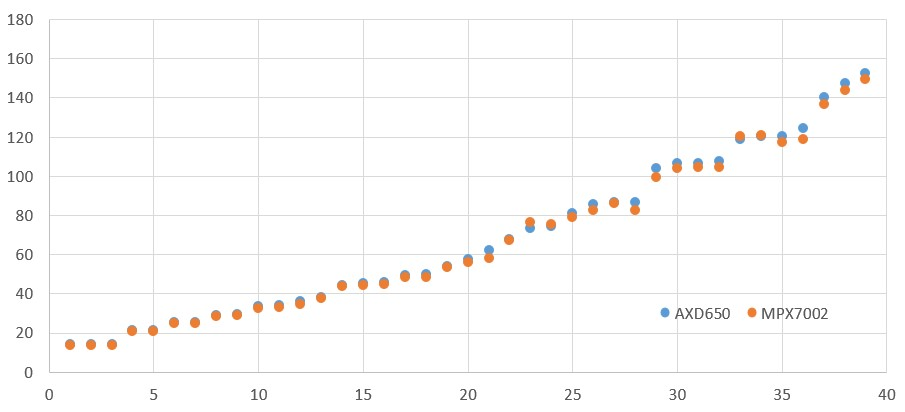
\includegraphics[scale=0.5]{condifpres.jpg}
	\captionof{figure}{Contraste de valores de presión diferencial del MPX7002}
	\label{fig:condifpres}
\end{figure}

\begin{table}[H]%diferencia de presion
		\centering
		\begin{tabular}{|r|r|r}
			\cline{1-2}
			\multicolumn{2}{|c|}{Diferencia de presión {[}Pa{]}} & \multicolumn{1}{c}{} \\ \hline
			\multicolumn{1}{|c|}{\textbf{AXD650}} & \multicolumn{1}{c|}{\textbf{MPX7002}} & \multicolumn{1}{c|}{\textbf{E$_r$}} \\ \hline
			14 & 13,51 & \multicolumn{1}{r|}{3,50\%} \\ \hline
			14 & 13,76 & \multicolumn{1}{r|}{1,71\%} \\ \hline
			14 & 13,76 & \multicolumn{1}{r|}{1,71\%} \\ \hline
			21,3 & 20,88 & \multicolumn{1}{r|}{1,97\%} \\ \hline
			21,5 & 20,88 & \multicolumn{1}{r|}{2,88\%} \\ \hline
			25,3 & 24,8 & \multicolumn{1}{r|}{1,98\%} \\ \hline
			25,4 & 24,8 & \multicolumn{1}{r|}{2,36\%} \\ \hline
			28,9 & 28,51 & \multicolumn{1}{r|}{1,35\%} \\ \hline
			29,3 & 28,8 & \multicolumn{1}{r|}{1,71\%} \\ \hline
			33,4 & 32,5 & \multicolumn{1}{r|}{2,69\%} \\ \hline
			34,1 & 32,88 & \multicolumn{1}{r|}{3,58\%} \\ \hline
			35,9 & 34,8 & \multicolumn{1}{r|}{3,06\%} \\ \hline
			38,1 & 37,38 & \multicolumn{1}{r|}{1,89\%} \\ \hline
			44,2 & 43,88 & \multicolumn{1}{r|}{0,72\%} \\ \hline
			45,5 & 44,5 & \multicolumn{1}{r|}{2,20\%} \\ \hline
			45,9 & 44,88 & \multicolumn{1}{r|}{2,22\%} \\ \hline
			49,4 & 48,51 & \multicolumn{1}{r|}{1,80\%} \\ \hline
			49,9 & 48,51 & \multicolumn{1}{r|}{2,79\%} \\ \hline
			54 & 53,26 & \multicolumn{1}{r|}{1,37\%} \\ \hline
			57,7 & 56,2 & \multicolumn{1}{r|}{2,60\%} \\ \hline
			62,1 & 58,13 & \multicolumn{1}{r|}{6,39\%} \\ \hline
			68 & 67,13 & \multicolumn{1}{r|}{1,28\%} \\ \hline
			73,4 & 76,6 & \multicolumn{1}{r|}{-4,36\%} \\ \hline
			74,3 & 75,26 & \multicolumn{1}{r|}{-1,29\%} \\ \hline
			81,1 & 79,01 & \multicolumn{1}{r|}{2,58\%} \\ \hline
			85,5 & 82,76 & \multicolumn{1}{r|}{3,20\%} \\ \hline
			86,4 & 86,1 & \multicolumn{1}{r|}{0,35\%} \\ \hline
			86,8 & 82,63 & \multicolumn{1}{r|}{4,80\%} \\ \hline
			104 & 99,26 & \multicolumn{1}{r|}{4,56\%} \\ \hline
			106,5 & 104,13 & \multicolumn{1}{r|}{2,23\%} \\ \hline
			106,8 & 104,5 & \multicolumn{1}{r|}{2,15\%} \\ \hline
			107,8 & 104,63 & \multicolumn{1}{r|}{2,94\%} \\ \hline
			118,8 & 120,13 & \multicolumn{1}{r|}{-1,12\%} \\ \hline
			120,4 & 120,6 & \multicolumn{1}{r|}{-0,17\%} \\ \hline
			120,5 & 117,38 & \multicolumn{1}{r|}{2,59\%} \\ \hline
			124,4 & 119 & \multicolumn{1}{r|}{4,34\%} \\ \hline
			140,1 & 136,6 & \multicolumn{1}{r|}{2,50\%} \\ \hline
			147,2 & 143,8 & \multicolumn{1}{r|}{2,31\%} \\ \hline
			152,7 & 149,38 & \multicolumn{1}{r|}{2,17\%} \\ \hline
		\end{tabular}
	\caption{Contraste de los valores de presión diferencial.}
	\label{difpres}

\end{table}

\subsection{Contrastación de velocidades}
Como prueba final se decidió realizar la contrastación de la velocidad estimada contra la velocidad de otro dispositivo. Para esto, se procedió a colocar en el interior del túnel un anemómetro digital \textbf{Avm-01 -\textit{ Prova}} perteneciente al laboratorio. A medida que se efectuaban las  pruebas, se realizó de manera simultanea la filmación del anemómetro y la pantalla con la aplicación realizada para luego unir ambos videos y poder tomar valores al mismo tiempo (Figura \ref{fig:capt}).

Estos valores fueron volcados a la tabla \ref{difvel} y luego graficados para observar posibles errores(Figura \ref{fig:vel_muestras}).

\begin{table}[H]
	\centering
	\begin{tabular}{|r|r|r}
		\cline{1-2}
		\multicolumn{2}{|c|}{velocidad {[}m/s{]}} & \multicolumn{1}{l}{} \\ \hline
		\multicolumn{1}{|c|}{\textbf{estimada}} & \multicolumn{1}{c|}{\textbf{anemómetro}} & \multicolumn{1}{c|}{\textbf{E$_r$}} \\ \hline
		4,6 & 4,7 & \multicolumn{1}{r|}{2,13\%} \\ \hline
		4,7 & 4,7 & \multicolumn{1}{r|}{0,00\%} \\ \hline
		4,8 & 4,7 & \multicolumn{1}{r|}{-2,13\%} \\ \hline
		5 & 5 & \multicolumn{1}{r|}{0,00\%} \\ \hline
		5,9 & 6 & \multicolumn{1}{r|}{1,67\%} \\ \hline
		6 & 6,1 & \multicolumn{1}{r|}{1,64\%} \\ \hline
		6,1 & 6,2 & \multicolumn{1}{r|}{1,61\%} \\ \hline
		7,8 & 7,8 & \multicolumn{1}{r|}{0,00\%} \\ \hline
		7,9 & 8 & \multicolumn{1}{r|}{1,25\%} \\ \hline
		8,9 & 9,2 & \multicolumn{1}{r|}{3,26\%} \\ \hline
		9,1 & 9,3 & \multicolumn{1}{r|}{2,15\%} \\ \hline
		11,9 & 12,4 & \multicolumn{1}{r|}{4,03\%} \\ \hline
		12 & 12,3 & \multicolumn{1}{r|}{2,44\%} \\ \hline
		12 & 12,4 & \multicolumn{1}{r|}{3,23\%} \\ \hline
		12,2 & 12,4 & \multicolumn{1}{r|}{1,61\%} \\ \hline
		12,3 & 12,5 & \multicolumn{1}{r|}{1,60\%} \\ \hline
		13,7 & 14,5 & \multicolumn{1}{r|}{5,52\%} \\ \hline
		13,8 & 14,4 & \multicolumn{1}{r|}{4,17\%} \\ \hline
		13,8 & 14,4 & \multicolumn{1}{r|}{4,17\%} \\ \hline
		13,9 & 14,3 & \multicolumn{1}{r|}{2,80\%} \\ \hline
		14 & 14,4 & \multicolumn{1}{r|}{2,78\%} \\ \hline
		14,2 & 14,5 & \multicolumn{1}{r|}{2,07\%} \\ \hline
		14,3 & 14,9 & \multicolumn{1}{r|}{4,03\%} \\ \hline
		14,7 & 15,6 & \multicolumn{1}{r|}{5,77\%} \\ \hline
		14,8 & 15,7 & \multicolumn{1}{r|}{5,73\%} \\ \hline
		14,9 & 15,5 & \multicolumn{1}{r|}{3,87\%} \\ \hline
		14,9 & 15,8 & \multicolumn{1}{r|}{5,70\%} \\ \hline
		15 & 15,7 & \multicolumn{1}{r|}{4,46\%} \\ \hline
		15,1 & 16,2 & \multicolumn{1}{r|}{6,79\%} \\ \hline
		15,3 & 16,3 & \multicolumn{1}{r|}{6,13\%} \\ \hline
	\end{tabular}
	\caption{Contraste de los valores de velocidad.}
\label{difvel}
\end{table}


\begin{figure}[H]
	\centering
	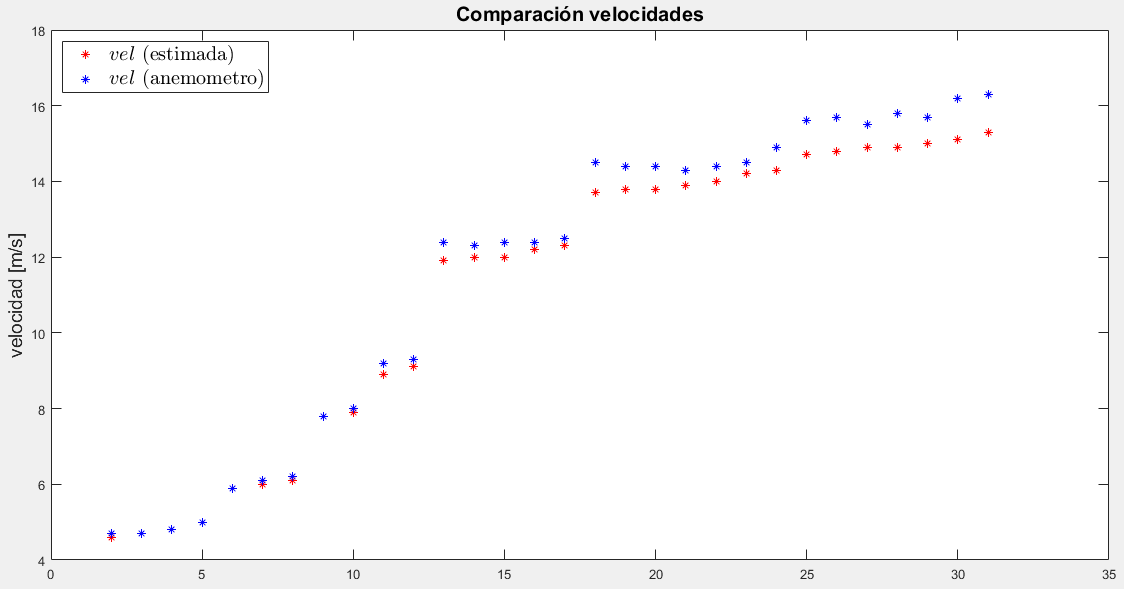
\includegraphics[scale=0.5]{vel_muestras.png}
	\captionof{figure}{Contraste de valores de velocidad estimada}
	\label{fig:vel_muestras}
\end{figure}


Al examinar la tabla y el gráfico se observa errores mayores a medida que las velocidades se incrementan.

\begin{figure}[H]
	\centering
	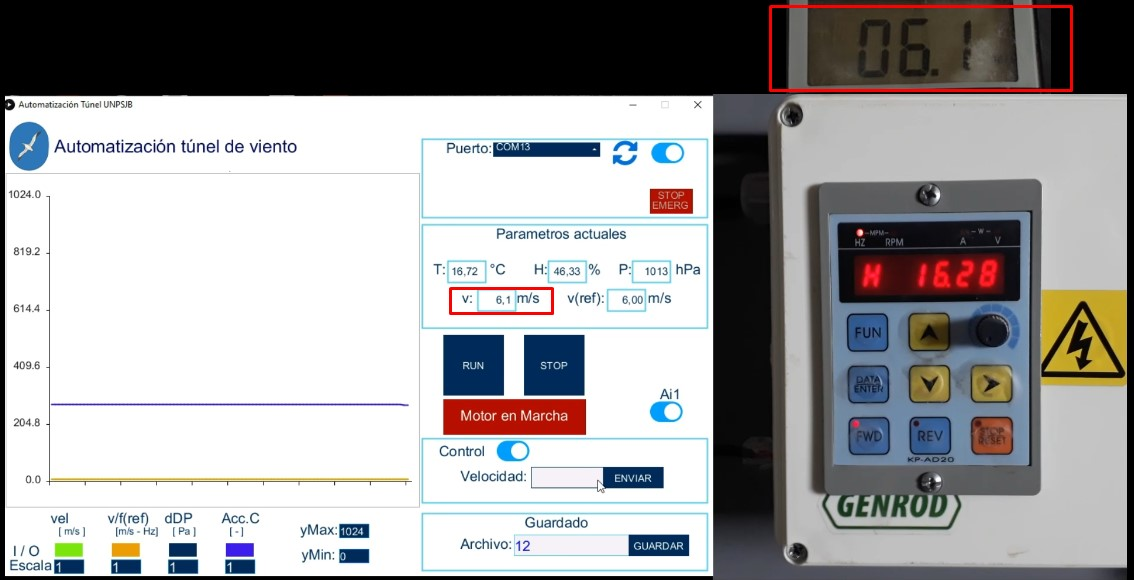
\includegraphics[scale=0.5]{captura.jpg}
	\captionof{figure}{Captura de pantalla del video utilizado para la realización del contraste de velocidad}
	\label{fig:capt}
\end{figure}



	\newpage
	\section{Implementación} 
	\subsection{Planos eléctricos}
NOSE

\subsection{Implementación física final}
NUEVA PLACA

\subsection{HMI}
NOSE
		\newpage
	\section{Recomendaciones futuras}
	\begin{itemize}
	\item Utilización de un cable UTP mallado para mejorar interferencias que puedan producirse entre el variador y el $\mu$C.
\item Realización de una aplicación con \textit{bluetooth} para Android.
\item Automatización de las compuertas laterales utilizadas para generar perturbaciones al sistema.
\item Realización de una nueva GUI según necesidades del laboratorio.
\item Realización de distintas señales de control para diversos rangos de velocidades.
\item Realización de una nueva parte del programa del microcontrolador para que puedan ser cargadas otros tipos de perfiles de velocidad (rampas, funciones cuadráticas, etc)
\item Adquisición de un nuevo motor con tecnología actual y lograr bajar el tiempo de los parámetros de aceleración y desaceleración (F35 y F36).
\end{itemize}
	\newpage
	\section{Conclusión}
	Siempre que se habla de control de procesos industriales, los PLC son los dispositivos más adecuados para el desarrollo de sistemas de este tipo. Para nosotros fue un desafío utilizar un microcontrolador ($\mu$C) para llevar a cabo el control de velocidad del túnel de nuestra Universidad.

Al utilizar un $\mu$C no se tiene la robustez que un dispositivo industrial posee, pero sin embargo, logramos una comunicación estable y un control eficaz sobre el variador de velocidad. Además, al disponer de esta opción, los costos de diseño e implementación son más económicos contra el empleo de dispositivos industriales.

Si bien es cierto que teníamos conocimientos básicos en el uso de herramientas de programación, el proyecto de automatización del túnel fue un aprendizaje que sumó a nuestros conocimientos nuevos lenguajes de programación, técnicas de trabajo y adicionalmente, saberes sobre el funcionamiento de los dispositivos que realizan las acciones sobre el proceso: motores, variadores de velocidad, señales analógicas y digitales, etc. 

La realización de una aplicación que permite la adquisición de datos,  la visualización de los mismos en tiempo real, el guardado de éstos en tablas, y la realización de gráficos de los datos guardados, hacen al sistema flexible tanto para la realización de los ensayos en el túnel de viento, como para el análisis posterior de los datos medidos. Además, se posibilitó el manejo remoto del variador de velocidad, y un control de lazo cerrado, en reemplazo de la utilización del panel frontal del variador, y del control de lazo abierto.

Como resultado final, se obtuvo un control de velocidad, en donde las mediciones obtenidas fueron cercanas a los valores estimados por el Laboratorio Mecánica de Fluidos, lo que ayudaría a minimizar la cantidad de procesos para la determinación de velocidad durante la contrastación de anemómetros. Además, nuestro controlador permitiría realizar nuevas experiencias de laboratorio de asignaturas afines a la temática, ya que se podrían generar cambios de velocidad controlados, perfiles de viento determinados, simular ráfagas, entre otras aplicaciones.


	

		\newpage
	\section{Bibliografia}


\printbibliography

\newpage

\appendix
\clearpage
%\addappheadtotoc
\appendixpage
%\section*{Anexos}

\section{Descargas}
El siguiente proyecto con sus respectivos archivos se encuentra para realizar la descarga en el repositorio GITHUB.
poner la tarjeta como imagen
\url{https://opengraph.githubassets.com/1/UNPSJB-YC/Automatizacion_Tunel_UNPSJB}

\url{https://github.com/UNPSJB-YC/Automatizacion_Tunel_UNPSJB}
\newpage
\section{Manual de usuario de la aplicación}
\subsection{Requerimientos del sistema}
\begin{itemize}
	\item Windows
	\item Driver de comunicación serial para CH340 \url{https://electrocrea.com/blogs/tutoriales/como-instalar-driver-ch340-para-arduinos-genericos}
\end{itemize}


\subsection{Puesta en marcha}
\begin{enumerate}
	\item Alimente variador de velocidad y el motor.
	\item Enchufe a 220V el cable de alimentación que sale de la implementación física.
	\item Conecte el cable serial USB que sale de la implementación física.
	\item Ejecute el programa “NOMBRE.EXE”
	\item Seleccione el puerto dónde se encuentra conectado el microcontrolador.
	\item Active el puerto.
	\item Al inicializar el puerto, el microcontrolador comienza a entregar valores a la aplicación por lo que se observa THP, velocidad estimada y frecuencia de referencia. 
	
\end{enumerate}

\begin{figure}[H]
	\centering
	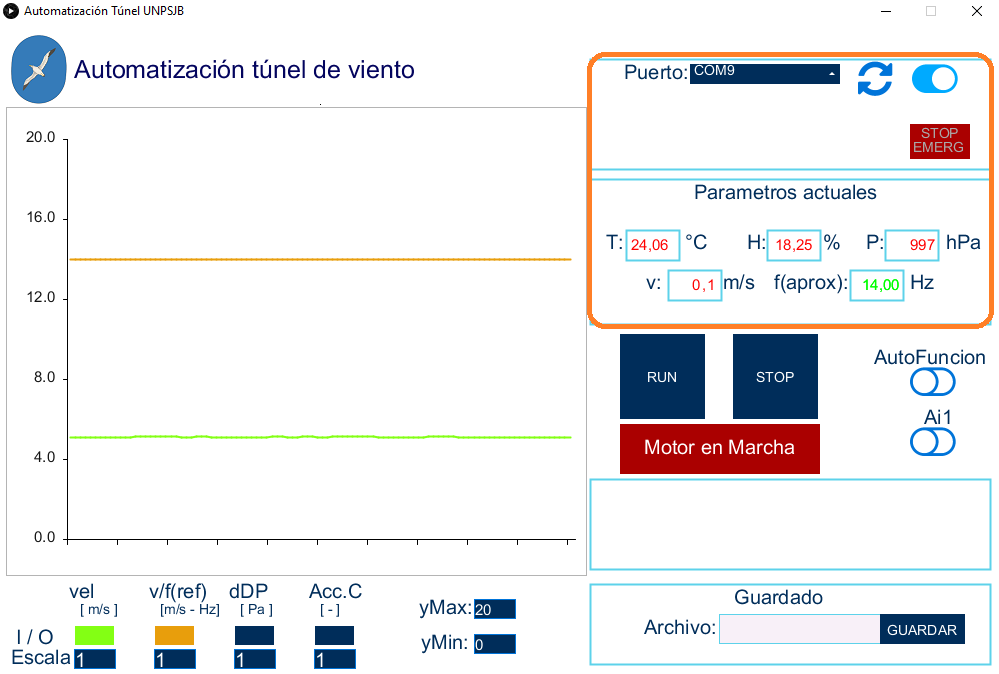
\includegraphics[scale=0.5]{capt2.png}
	\captionof{figure}{Puerto activado. Aplicación leyendo valores del $\mu$C.}
	\label{fig:capt2}
\end{figure}



\subsection{Gráfico en tiempo real}
\subsubsection{	Visibilidad de las señales en tiempo real}
En la parte izquierda inferior del programa, se puede activar o desactivar la visibilidad de las variables a observar en tiempo real, solo basta realizar un click en los rectángulos, y estos al estar activados se colocarán del color correspondiente a la señal a observar.

\subsubsection{Escala}
En la parte inferior se encontrará “Escala” donde se establece la escala correspondiente de cada señal.
\begin{enumerate}
	\item Realice click en el interior del rectángulo
	\item Borre el número que posee y colocar el valor nuevo a ingresar.
	\item Presione “enter”.
	\item La escala de la señal elegida será modificada.
	
\end{enumerate}

\textbf{Ejemplo de escala:}

Si se coloca en una señal “10”, la variable observada en tiempo real estará aumentada 10 veces.

\subsubsection{Límite del eje vertical}
El eje vertical del gráfico en tiempo real puede ser modificado según necesidad.

\begin{enumerate}
	\item Realice click en el interior del rectángulo.
	\item Borre el número que posee y colocar el valor nuevo a ingresar.
	\item Presione “enter”.
	\item El eje “vertical” se verá modificado.
	
\end{enumerate}


\begin{figure}[H]
	\centering
	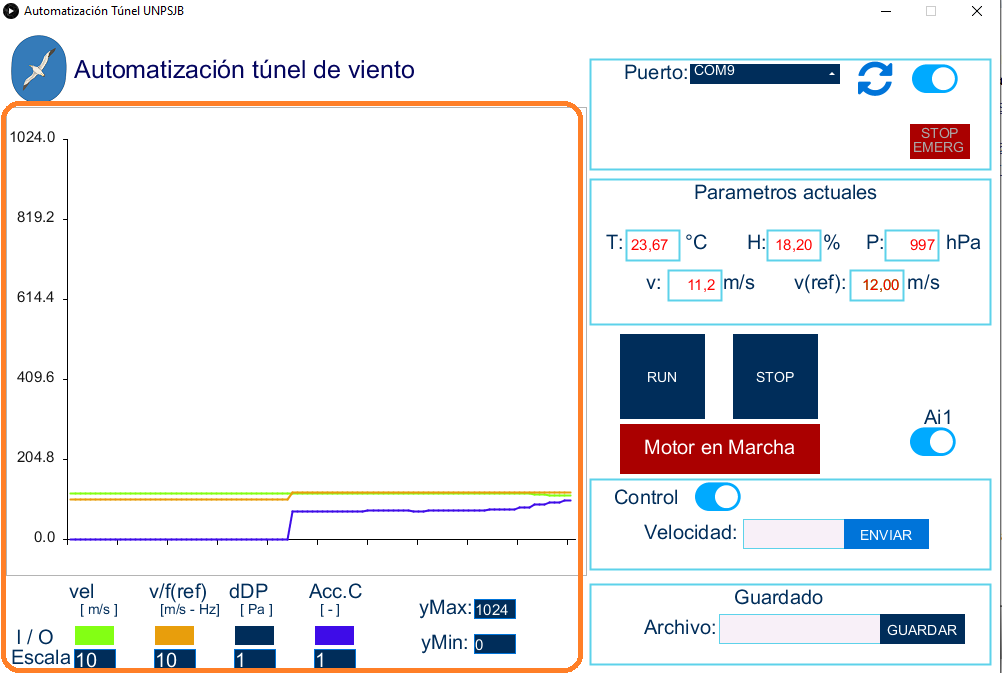
\includegraphics[scale=0.5]{capt3.png}
	\captionof{figure}{Gráfico en tiempo real}
	\label{fig:capt3}
\end{figure}

\subsection{Autofunción}
El modo de autofunción carga un archivo “.csv” que se encuentra dentro de la carpeta “autofun”. El archivo “.csv” posee los datos pertenecientes a los escalones de velocidad deseados y el tiempo de ejecución de cada uno.

\begin{figure}[htb]
	\centering
	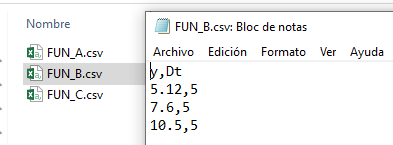
\includegraphics[scale=0.7]{carpcsv.png}
	\captionof{figure}{Archivos dentro de la carpeta "autofun"}
	\label{fig:autof2}
\end{figure}


El archivo tiene que tener el formato observado en la Tabla \ref{tab:formcsv}, donde se ve que posee un encabezado. Si se desea que la velocidad sea un número decimal, este debe ir con punto. 
\begin{table}[h]
	\centering
	\begin{tabular}{|l|}
		\hline
		y,Dt \\ \hline
		y1,Dt1 \\ \hline
		y2,Dt2 \\ \hline
		y3,Dt3 \\ \hline
	\end{tabular}
	
	\caption{Formato .csv}
	\label{tab:formcsv}
\end{table}

Mientras que se esté realizando este programa aparecerá una señal visual debajo del botón abrir. (Figura \ref{fig:autof1})

\begin{figure}[htb]
	\centering
	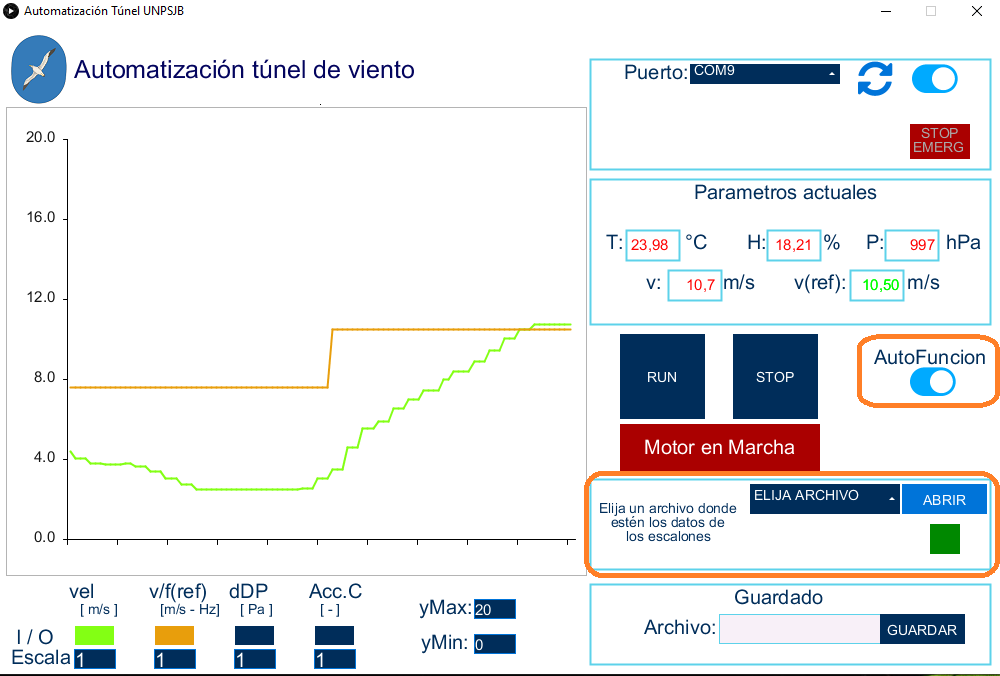
\includegraphics[scale=0.5]{capt1.png}
	\captionof{figure}{Aplicación funcionando en modo Autofunción}
	\label{fig:autof1}
\end{figure}



\subsection{Ai1}
\subsubsection{Control desactivado}
Al utilizar este modo de funcionamiento, se puede ingresar un valor aproximado de frecuencia. El lazo de control estará abierto.

\subsubsection{Control activado}
El lazo de control estará activado, ante perturbaciones el sistema tiende a establecerse a la velocidad estipulada. Para estipular la velocidad se debe presionar sobre la caja de “velocidad” ingresar un valor y presionar sobre el botón “enviar”

\subsection{Encendido/ apagado del motor}
El encendido/ apagado del motor se puede realizar de dos formas:
\subsubsection{Panel frontal}
Si el parámetro F7 del variado de velocidad se encuentra en “0”, la marcha y parada del motor será realizada por los botones físicos el panel frontal.
\subsubsection{Aplicación}
Si el parámetro F7 del variador de velocidad se encuentra en “1”, la marcha y parada del motor será realizada por los botones propios de la aplicación.


\subsection{Guardado de datos}
Al colocar un nombre y presionar la tecla guardar, se generará un archivo “.csv” con los datos que el microcontrolador capturó cada aproximadamente 55ms. 

\textbf{\textit{Alerta:}} Una vez que se presiona la tecla guardar o el puerto se cierra los datos son borrados y se comenzará una nueva tabla.

\begin{figure}[H]
	\centering
	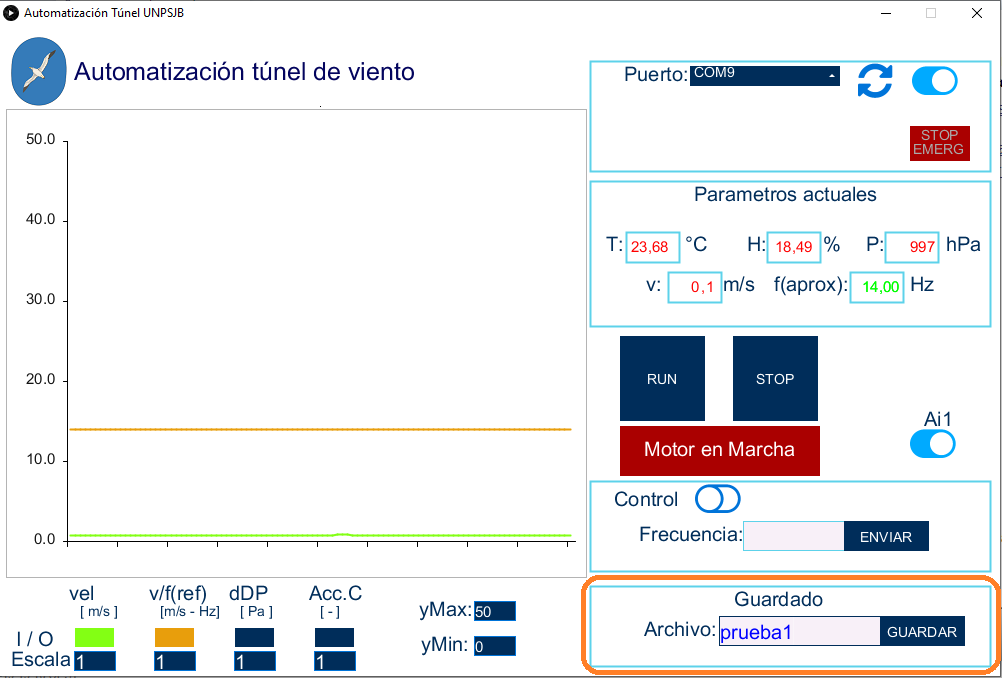
\includegraphics[scale=0.5]{capt4.png}
	\captionof{figure}{Guardado de datos}
	\label{fig:capt4}
\end{figure}


\subsection{Lectura de datos obtenidos}
El encabezado de la tabla (Figura \ref{fig:capt5}) muestra las siguientes leyendas:

\begin{itemize}
	\item \textit{Muestra:} número de muestra tomada
	\item \textit{Tiempo:} tiempo desde el inicio del puerto serie [ms].
	\item \textit{Temp:} temperatura ambiente [$^{\circ}$ C].
	\item \textit{Hum:} humedad relativa del ambiente [\%].
	\item \textit{Pres:} presión atmosférica [hPa].
	\item \textit{Den:} densidad estimada por el microcontrolador [$kg/m^3$].
	\item \textit{DP:} diferencia de presión medida a través del MPX7002 en conjunto con ADS1115 [Pa]
	\item \textit{Ref:} Valor de frecuencia o velocidad preestablecida [Hz ó m/s].
	\item \textit{VelFrec:} Velocidad del aire estimada [m/s].
	\item \textit{PWM:} señal de acción de control.
	\item \textit{Control:} señal de que el lazo de control está cerrado.
	\item \textit{Error:} error entre la velocidad estimada y la de referencia.
	\item \textit{ESTADOvariador:} estado encendido/apagado del motor.
	\item \textit{ERRORvariador:} indicación de algún error del variador de velocidad.
	\item \textit{TiempoRel:} indica tiempo desde el ultimo guardado de datos.
	\item \textit{ControlAutomatico:} indicación de comienzo y fin del control automático.
		
\end{itemize}

Para hacer lectura o interpretación de los datos se recomienda utilizar el script de matlab \fcolorbox{red}{yellow}{“NOMBRE DEL ARCHIVO DE MATLAB”}

\begin{figure}[H]
	\centering
	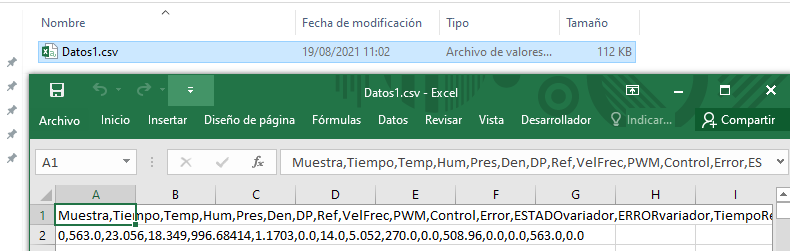
\includegraphics[scale=0.5]{capt5.png}
	\captionof{figure}{Archivo .csv generado}
	\label{fig:capt5}
\end{figure}

\subsection{Falla externa}
	Al presionar el botón de “Falla externa” el $\mu$C enviará una señal al variador y el sistema se detendrá.

\newpage
\section{Código Arduino}
\newpage
\section{Código Processing}
\newpage
\section{Código Matlab}






\end{document}